\documentclass[10pt]{report}

%opening
\title{Automated Checking of Implicit Assumptions on Textual Data } 
\author{Radwa Sherif Abdelbar \\
	 Supervisors: Dr. Caterina Urban, Alexandra Bugariu \\ Prof. Dr. Peter M{\"u}ller}
\usepackage{titlesec}
\usepackage{tikz}
\usepackage[style=numeric, maxbibnames=99, sorting=none]{biblatex}
\usepackage{amsfonts}
\usepackage{amsmath}
\usepackage{stmaryrd}
\usepackage{amsmath}
\usepackage{amsfonts}
\usepackage{listings}
\usepackage{syntax}
\usepackage{algorithm}
\usepackage[noend]{algpseudocode}
\usepackage[T1]{fontenc}
\usepackage{setspace}
\usepackage{graphicx}
\usepackage{url}
\usepackage{pdfpages}
\usepackage{pgfplots}
\usepackage{subcaption}
\usepackage{epstopdf}

\addbibresource{bachelors-thesis.bib}

\lstdefinestyle{mystyle}{
	numberstyle=\small,
	breakatwhitespace=false,         
	breaklines=true,                 
	captionpos=b,                    
	keepspaces=true,                 
	numbers=left,                    
	numbersep=5pt,                  
	showspaces=false,                
	showstringspaces=false,
	showtabs=false,                  
	tabsize=2,
	frame=single
}
\lstset{style=mystyle}

\titleformat{\chapter}{\normalfont\huge\bf}{\thechapter}{20pt}{\huge\bf}
\def\changemargin#1#2{\list{}{\rightmargin#2\leftmargin#1}\item[]}
\let\endchangemargin=\endlist

\begin{document}

\begin{titlepage}
	\begin{center}
		

		\begin{flushleft}
		
\includegraphics[width=0.4\textwidth]{ETHlogo.pdf}	
		\end{flushleft}
		\vspace*{-1.5cm}
		\begin{flushright}
			\includegraphics[width=0.3\textwidth]{GUC.eps}
		\end{flushright}
		\vspace*{1.5cm}		
		\LARGE{Automated Checking of Implicit Assumptions on Textual Data }
		
		\vspace{0.8cm}
		\normalsize{\textbf{Bachelor's Thesis}}
		
		\vspace{1.5cm}
		
		Radwa Sherif Abdelbar
		
		
	
		
		\vspace{2cm}
		
		
		Chair of Programming Methodology\\
		Department of Computer Science\\
		ETH Zurich\\
		2018
		
		\vfill
		\textbf{Supervisors:}\\
		Dr. Caterina Urban \\
		Alexandra Bugariu \\
		Prof. Dr. Peter M{\"u}ller
		
	\end{center}
\end{titlepage}
\pagebreak
\thispagestyle{empty}
\vspace*{10cm}
\begin{flushright}
	%\textit{To my grandfather,\\
	%whose humor, energy and affection I will always miss}
\end{flushright}

\pagebreak
\thispagestyle{empty}
\begin{center}
	\large{\textbf{Acknowledgements}} \\
\end{center}
%I am infinitely grateful to my supervisors, Dr. Caterina Urban and Alexandra Bugariu, who have provided me with all the support and guidance I needed to complete this project. Thank you for everything you have taught me over the past six months. I could not have hoped for better supervision. \\

I am also very grateful Prof. Dr. Peter M{\"u}ller for the opportunity to work on this project and to be part of a great research environment for half a year. \\

I would also like to thank the lecturers and teaching assistants at the Computer Science Department of the German University in Cairo for everything they have taught me during my studies and for sparking my interest in Computer Science. \\

I am grateful to Gagandeep Singh for helping me incorporate his work on numerical analysis into my work, to Marco Eilers for helping me with a challenging part of my implementation and to J{\'e}r{\^o}me Dohrau for his helpful remarks on my theoretical work. \\

There are no sufficient words with which to express my gratitude to my mother and father whose love and support have shaped my life and whose unwavering faith in me propels me to pursue my dreams. May I always make you proud. \\

I would have never been able to finish this work without the support, encouragement and prayers I recieved from my family and friends in Egypt.\\ 

I am grateful for the frienship of Karin Wenger who showed me around in Switzerland and made my time here unforgettable. \\

Finally, I am grateful to the members of the Chair of Programming Methodoloy at ETH Zurich whose friendly and welcoming attitude made me feel at home as a member of their group for six months. \\



\begin{abstract}
One of the main problems faced by data scientists in today's world is the challenge of finding and correcting errors in datasets before running their algorithms on them. 

The aim of this thesis is to present a mechanism that helps a user locate and correct errors in a data file that is read as input by a certain program. We use static analysis to build a generic framework that can make use of existing abstract domains to infer the implicit assumptions that a program makes about the data it reads as input such that if those assumptions are violated the program will raise an error. We create an instance of our analysis using three abstract domains and used it to track assumptions on numerical and string variables. Then we design an input checker that scans a data file and flags the values that violate those assumptions. We implemented our analysis and checker for Python programs and integrated them into a tool which we implemented as an IDE plug-in. 

We evaluated our static analysis by manually checking the assumptions it infers against manually computer assumptions and found that it is sound in all cases and precise in approximately 60\% of the cases and that the precision can be improved either by using more powerful domains in the analysis or by modifying the design of the analysis itself. 

We conducted a user study among 10 users from both Computer Science and non-Computer Science backgrounds to evaluate the usability of our tool. Our results show that the tool helps users find errors in the input data in less time then they took to do the same without the tool and with less reported frustration. 

 
\end{abstract}

\tableofcontents{}


\chapter{Introduction}

Today, we live in a world that produces tremendous amounts of data on a daily basis. The extensive use of social media websites and the digitization of traditional services such as banking, retail and publishing guarantees the existence of large datasets that are available to service providers. In addition to business, technological advancements have created an abundance of data in many fields of scientific research such as the genomic data created by efficient Deoxyribonucleic acid (DNA) sequencing or raw images of celestial bodies that are captured by modern telescopes \cite{blei2017science}. 

This abundance of data, along with the rapid development in new data science techniques and methods to organize, analyze and detect patterns in large datasets, creates new and unique opportunities for experts in different domains. For example, it enables businesses to predict future customer behavior or medical researcher to associate the presence of a specific gene in the human DNA with susceptibility to certain diseases. 

These advantages, however, are not achieved without challenges or difficulties. The datasets processed by data science algorithms are typically very large in size and could be obtained from various sources or maintained on different machines. For these reasons, they are likely to contain errors and inconsistencies. 

In the field of data science, raw data, that is data as it is collected from the source and stored on some storage medium (e.g. database or cloud), is not usually usable as is. A recent survey among data scientists \cite{kaggle} shows them to cite ``dirty data'' as one of the most challenging aspects of their work. Dirty data, as defined in \cite{dirty-data}, is data that is wrong, missing or not represented according to a known standard such as non-standard representation of time and date.

Before feeding the data into a data science program, it must be cleansed and the erroneous values must be corrected. Many tools have been introduced to achieve this goal. For example, \cite{cleaning} lists some data cleaning approaches and some of the tools which implement them. Data profiling tools, for instance, are specialized in collecting metadata about each attribute of the input data, this metadata is then used to detect errors in the data. On the other hand, data mining tools are concerned with inferring relationships between different data fields and checking integrity constraints among attributes. Another category of tools are domain specific, such as tools that focus on validating and formatting names and addresses, and others that specialize in duplicate elimination.  

In this thesis, we present an approach to detect incorrect input data with respect to a given data science program. Unlike the data-cleaning tools mentioned above, our method does not perform computations on the dataset directly. This is advantageous in cases where the data is confidential and therefore cannot be shared with third parties to perform data cleaning. Instead, we design a static analysis that analyzes the source code of the program in order to find out the implicit assumptions that the program makes about the input data that it reads such that if these assumptions are violated the program will crash These assumptions represent the pre-conditions that must be satisfied so that the program runs without producing errors. Our analysis will compute an over-approximation of these pre-conditions. In other words, if there is a set of accepted values that will allow the program to run without raising an error, the set of values that our analysis computes will contain all the accepted values, but it might contain some extra values that will cause the program to raise errors. That is, the pre-conditions we compute are necessary but not sufficient for the program to terminate without crashing. 

We then design an input checker that looks for values in an input data file that violate the assumptions computed by the analysis. If that is the case, the wrong input values are flagged as errors so that the user can correct them. We implement our analysis and input checker for Python programs and integrate them into a tool that can be used directly by domain experts on their data. 
\begin{lstlisting} [language = Python, label=first, caption=Example of Program with Assumptions on String and Integer Data] 
	sequence_length: int = int(input())
	count_a: int = 0
	count_c: int = 0
	count_g: int = 0
	count_t: int = 0
	for i in range(sequence_length):
		base: str = input()
		if base == 'A':
			count_a: int = count_a + 1
		elif base == 'C':
			count_c: int = count_c + 1
		elif base == 'G':
			count_g: int = count_g + 1
		elif base == 'T':
			count_t: int = count_t + 1
		else:
			raise ValueError
			
\end{lstlisting} 

To elaborate further on what we aim to achieve in this thesis, let us examine the program in Listing 1. This program aims to read a DNA sequence and count the frequency of occurrence of each nucleotide. It first reads the length of the sequence (line 1), then since the only possible nucleotides in a DNA sequence are represented by the letters A, C, G and T, it sets a frequency counter for each of these nucleotides (lines 2-5). Then the program iterates through the sequence, reading one letter per line and incrementing the corresponding counter variable. If it encounters a letter that is neither A, C, G or T, it raises an error (line 17) because it \textit{assumes} that, in an ideal scenario, no value in the input file will be outside this set of letters.  

Our aim, thus, is not to perform computations on the input data based on the known fact that the human DNA contains only A, C, G and T bases and to cleanse the wrong values. Rather, we turn our attention to the program that will run on the data and try to answer the question: what does this program \textit{assume} about its input data such that if those assumptions are not fulfilled, the program will raise an error? For our analysis to compute a successful over-approximation, it must always include the values `A', `C', `G' and `T' in the set of accepted values it produces. However, it may include some other values as well. 

In section \ref{theoretical}, we present the theoretical aspects upon which the work of this thesis is based. In section \ref{analysis}, we explain the design of our static analysis and its different components in more detail. In section \ref{implementation}, we give an overview of how our analysis and input checker were implemented and integrated into an IDE plug-in. We evaluate our approach in section \ref{evaluation}, related work is presented in section \ref{related}, finally, the conclusion and possible future work are to be found in section \ref{conclusion}. 

\section{Theoretical Background} \label{theoretical}

In this section we present the basic theoretical concepts which we use in our work. 

\subsection{Static Analysis}
Static analysis is the analysis of a program, without executing it, in order to infer some properties about the program's behaviour. Since, as per Rice's theorem, it is generally impossible to infer with absolute certainty that a non-trivial property holds for all executions of a program, static analysis aims to approximate the behaviour of a program by creating a model of the program and analyzing this model in all of the program's execution paths.  

\subsection{Abstract Interpretation}
The theory of Abstract Interpretation \cite{cousot} is a general theory that allows for creating mathematically sound approximations of the behaviour of a program. It was created by Patrick Cousot and Radhia Cousot as a unifying framework for static analysis.  

According to Abstract Interpretation, a program can have several semantics, that is several mathematical descriptions of its behaviour. The \textbf{concrete semantics} is a mathematical formalization of the behaviour of a program in all possible executions and in all possible execution environments. The concrete semantics of a program is impossible to compute and therefore this makes it impossible to prove that a non-trivial property of a program holds in all its execution paths. The \textbf{abstract semantics}, on the other hand, represents the semantics of the program with respect to some chosen property while abstracting away the irrelevant details. The abstract semantics is a superset of the concrete semantics and therefore any property which holds for the abstract semantics is guaranteed to also hold for the concrete semantics. For example, the concrete semantics of a program can be the values which its numerical variables take, while an abstract semantics could be the signs of these variables or the ranges they can take.   

In order to use Abstract Interpretation for static analysis, we must define an abstract domain that represents the states of the program according to the abstract semantics. An abstract domain is usually represented as a complete lattice $ (D, \sqsubseteq, \sqcup, \sqcap, \bot, \top) $. $ D $ is the set of abstract elements which represent the state of the program in the abstract domain. The \textbf{partial order} $ \sqsubseteq $ is used to compare two elements of the domain: $ a \sqsubseteq b$ holds if $ a $ represents a more precise approximation of the concrete semantics than $ b $. The \textbf{join} operator $ \sqcup $ is used to compute the least upper bound of two abstract elements: $ a \sqcup b$ gives the element which represents the less precise approximation of the concrete semantics, the ``larger'' element. The \textbf{meet} operator $ \sqcap $ is used to compute the greatest lower bound of two abstract elements: $ a \sqcap b $ gives the element with the most precise approximation of the concrete semantics, the ``smaller'' element. The \textbf{minimum element} $ \bot $ represents an empty set in the concrete semantics, while the \textbf{maximum} element $ \top $ represents the set of all possible states in the concrete semantics. In case the domain is represented by a lattice of infinite height, it requires a \textbf{widening} $ \nabla $ which ensures that the analysis eventually reaches a fixed point.  

All the operators of an abstract domain must be defined such that their results preserve the soundness of the domain. That is, it must always remains the case that the elements resulting from these operators represent supersets of the concrete semantics. In section \ref{analysis}, we define the main abstract domain used in this thesis and its operators. 


\section{Contribution}

Our approach is based on the work done in \cite{madelin}. This work was focused on inferring assumptions on numerical values. They inferred assumptions on the types of these variables, the ranges they are allowed to take and simple relations between them. They developed a mechanism to store these assumptions in a structured manner and an input checker that checks the values in an input file against these assumptions. Their input checker was designed as a standalone tool. 

Since we would like to analyze more complex code examples that contain assumptions on both numerical and string values, such as Listing \ref{first}, we extend this approach to be more generic. Our approach is designed to be a generic framework which can keep track of assumptions on variables of any type. We also present a generic mechanism to store these assumptions. We create an instance of this generic framework that track assumptions on the types of variables, using the same mechanism as \cite{madelin}, as well as relational assumptions between numerical variables and assumptions on the characters contained in a string. Similar to \cite{madelin}, we design an input checker that checks a data file for values that violate these assumptions. Our input checker is implemented as an IDE plug-in for a better user experience. 

\chapter{Static Analysis Design} \label{analysis}
In this section, we present a detailed description of our static analysis. In the next section we present the concrete semantics which we use in our analysis. In section \ref{assumption-domain}, we describe our generic framework for inferring assumptions on input data as a top-level abstract domain. In section \ref{analysis-instance}, we describe three abstract domains, namely the Type Domain (section \ref{types}), the Octagon Domain (section \ref{octagon}) and the Character Inclusion Domain (section \ref{character}), which we use to create the instance of our generic framework that we use to demonstrate how our technique works throughout this thesis and which we also used for our implementation. 
\section{Concrete Domain} \label{concrete}

To define our concrete domain, we first define the following sets:
\begin{itemize}
	\item $\mathcal{L}$: the set of all program points in the program being analyzed. 
	\item $\mathcal{S}$: the set of all possible string values. 
	\item $\mathcal{V}$: the set of all program variables.
	\item$\wp(\mathcal{V} \rightarrow \mathcal{S})$: the set of environments mapping program variables to their possible values. 
	\item $\wp(\mathcal{S})^{*}$: the list of all possible values read as input from one program point onwards.  
\end{itemize}

We can then define our concrete domain as follows: 
\begin{center}
$\mathcal{L} \rightarrow \wp(\mathcal{V} \rightarrow \mathcal{S}) \times \wp(\mathcal{S})^{*}$
\end{center}

As indicated by the formula, our  concrete domain maps a program point to a set of environments mappings program variables to the values they are allowed to take and a list of input values which the program reads from this point onwards. Specifically, given a program, its concrete semantics is the set of values that its variables are allowed to take and the list of input values that it is allowed to read so that it terminates without errors.   

\section{The Assumption Abstract Domain} \label{assumption-domain}
We use the theory of Abstract Interpretation \cite{cousot} to design an abstract domain that over-approximates the concrete semantics defined in the previous section. In this context, over-approximation means that the constraints inferred by the analysis are necessary but not sufficient for the program to run without producing an error. If the input values violate those constraints, the program is guaranteed to produce an error. That is, we guarantee an absence of false-positives. However, if the input values satisfy all the constraints, the program might still produce an error. Our static analysis works backwards by starting at the final state of the program and analyzing all the execution paths of the program until it reaches the initial state. Since in the normal order of program execution a value is read as input first then the constraints upon it are imposed, it is intuitive for our analysis to traverse the program backwards, collecting the constraints that are imposed on program variables and then storing these constraints as assumptions on input values once these program variables are read as inputs. 

To examine the properties of our domain, let us consider the program in Listing 2, which performs the same operation as Listing 1, namely reading a DNA sequence and counting the frequency of every nucleotide, but on multiple sequences separated by a '.' or '\#' character. On line 1, the number of sequences is read. Lines 3 and 4 assert that we have at least one sequence in the file. Another addition in Listing 2 is the check that the sequence length is not greater than some maximum length on lines 7 and 8. 

There are multiple ways in which this program can produce an error. On line 1 if the value read cannot be cast to an integer, a error will be raised by Python. If the number of sequences is not positive (line 3), the length of each sequence is greater than the designated maximum sequence length, the sequence contains characters other than A, C, G and T (lines 15 through 24) or if the separator character is not a hash or a dot (line 26), the program raises a ValueError explicitly. 

It is obvious from this example that we need to track information about both numerical values and string values if we are to compute the set of allowed input values to this program. For example, we need to ensure that the relation $sequence\_length > max\_length$ holds and that the variable $base$ has only the characters in the set $\lbrace'A', 'C', 'G', 'T' \rbrace$. This cannot be achieved by running a conventional static analysis using only one abstract domain.

\begin{lstlisting} [language=Python, label=running, caption=Running Example]
	number_of_sequences: int = int(input())
	max_length: int = int(input())
	if number_of_sequences <= 0 :
		raise ValueError("Expecting at least one DNA sequence")
	for s in range(number_of_sequences):
		sequence_length: int = int(input())
		if sequence_length > max_length:
			raise ValueError
		A_count: int = 0
		C_count: int = 0
		G_count: int = 0
		T_count: int = 0
		for i in range(sequence_length):
			base: str = input()
			if base == 'A':
				A_count: int = A_count + 1
			elif base == 'C':
				C_count: int = C_count + 1
			elif base == 'G':
				G_count: int = G_count + 1
			elif base == 'T':
				T_count: int = T_count + 1
			else:
				raise ValueError
		separator: str = input()
		if separator == '.' or separator == '#':
			pass
		else:
			raise ValueError
\end{lstlisting}



Our abstract domain, which we call the Assumption Domain, is a generic domain that allows for the approximation of multiple program properties simultaneously. It is parametrized by a list of abstract domains which are independent of one another. For each step of the analysis, the Assumption Domain invokes the corresponding operator or transformation on each domain independently. We define $ SUBD $ to be a family of domains that can be used in our analysis. Any value domain can be a member of this family given that it defines extra operators that are described in \ref{sub-domains}. The Assumption Domain uses these domains to keep track of assumptions on the values of program variables. For example, in the case of Listing \ref{running}, we can use the Octagons Domain \cite{octagon} to keep track of the relations between numerical variables such as $sequence\_length \leq max\_length$ and the Character Inclusion Domain \cite{character} to keep track of the characters of the variable $base$.

Going back to Listing 2, if we trace a backward static analysis from line 24 to line 15 using the Character Inclusion Domain, which keeps track of the characters that a string contains, as a sub-domain, we will get that the variable $ base $ is allowed to contain only the characters 'A', 'C', 'G' and 'T'. When this variable is read as input on line 14, we need to store the assumption in some data structure. The same applies for the variable $ sequence\_length $. Tracing the analysis backwards using the Octagon Domain will give us the constraint $ sequence\_length \leq max\_length $. On line 6, when the variable is read as input, this constraint must be stored in a way that preserves its order among other inputs that the program reads in the course of its execution. More specifically, we need a data structure in which the assumptions about $ sequence\_length$ appear before those about $ base $.  We also need a data structure that indicates how many times an input value is read. For example, it needs to show that the variable $ base $ is read $ sequence\_length $ number of times. 

In our case, we choose this data structure to be a stack, in which every layer represents a scope of the program. Whenever the analysis enters a new branch or a loop, a new layer is pushed onto the stack. Inside of this scope, whenever a variable is read as input, we store its constraints in the top layer of the stack. When exiting a branch or a loop, the top layer is popped from the stack and combined with the layer below it in such a way that the assumptions appear in the order in which the inputs are read. In the case of exiting a loop, we define a mechanism to indicate how many times a group of assumptions is repeated. This way, at the end of the analysis, the stack will contain all the assumptions on the input values of the program in the correct order. We define the stack with further detail in section \ref{stack}. 

Given the previously mentioned properties, we introduce our domain formally below. \\
  

We define $STACK$ to be a set of all possible stacks which store assumptions on input values of the program.

We use the notation $ (X_{i})_{i=1}^{n} $ throughout this thesis to indicate a list of length $ n $. We use the symbol $ \oplus $ to denote list concatenation. \\

We can proceed to define the Assumption Domain formally. The soundness of the operators of the Assumption Domain follows from the soundness of the operators of the sub-domains and the stack: \\
\begin{center}
	$D \equiv SUBD^{n} \times STACK$\\	
\end{center}
\begin{itemize}
	\item An element $d \in \textsl{D} = \lbrace ((S_{i})_{i=1}^{n}, Q) \vert S_{i} \in SUBD \wedge Q \in STACK \rbrace$. Every element of this domain consists of a sequence of instances of sub-domains and a stack.
	\item A concretization function $\gamma_{D}(d) =( \bigcap\limits_{i=1}^{n}\gamma_{S_{i}}(S_{i}), \gamma_{STACK}(Q)).$ The concretization function gives a set of values that is a superset of the set of values allowed by the concrete domains. This applies to both the set of values that program variables are allowed to take, represented by the intersection of the concretization of the sub-domains, and the set of allowed input values, represented by the concretization of the stack. 
	 
	\item A partial order $\sqsubseteq_{D}$ such that $ ((S_{1,i})_{i=1}^{n}, Q_{1}) \sqsubseteq_{D} ((S_{2, i})_{i=1}^{n}, Q_{2}) \Longleftrightarrow $ \\ $\bigwedge\limits_{i=1}^{n}(S_{1,i} \sqsubseteq_{S_{i}} S_{2,i}) \wedge Q_{1} \sqsubseteq_{STACK} Q_{2} .$ An element $ d_{1} $ of $ D $ is small than or equal to another element $ d_{1} $ if and only if $ d_{1} $ represents a set of allowed input values that is smaller than or equal the set allowed input values by $ d_{2} $. 
	\item A minimum element $\bot_{D} = ((\bot_{S_{i}})_{i=1}^{n}, \bot_{STACK})$. This elements represents a state where there are no possible input values that are acceptable by the program. 
	\item A maximum element $\top_{D} =  ((\top_{S_{i}})_{i=1}^{n}, \top_{STACK})$. This represents the set of all possible input value without any constraints. 
	\item A join operator $\sqcup_{D}$ such that $ ((S_{1,i})_{i=1}^{n}, Q_{1}) \sqcup_{D} ((S_{2,i})_{i=1}^{n}, Q_{2}) = (((S_{1,i} \sqcup_{S_{i}} S_{2,i})_{i=1}^{n}, Q_{1} \sqcup_{STACK} Q_{2}))$. When joining two paths of the analysis, we must join the constraints computed by the analysis on both the program variables, by performing a pair-wise join on all the sub-domains and joining the two stacks $ Q_{1} $ and $ Q_{2} $. The soundness of this operator follows from the soundness of the join operators of the sub-domains and the join operator of the stack. The join operator of this domain is sound if the set of allowed values for program variables and the set of allowed input values to be read by the program produced from the join remain a subset of their counterparts in the concrete domain. This is achieved if the join operator of every sub-domain preserves soundness by producing a set of allowed values for program variables that is a superset of the set of allowed values produced by joining the two elements in the concrete domain $ (\gamma_{S_{i}}(S_{1,i}) \cup \gamma_{S_{i}}(S_{2,i}) \subseteq \gamma_{S_{i}}(S_{1, i} \sqcup_{S_{i}} S_{2,i})) $ and, similarly, the stack join produces a list of allowed input values that are element-wise superset of the list of allowed input values computed by joining the two stack in the concrete domain. We elaborate on the join of the stack in section \ref{stack}. 
	 
	\item A backward assignment operator $\llbracket X:=aexpr \rrbracket_{D} ((S_{i})_{i=1}^{n}, Q) =  ((\llbracket X:=aexpr \rrbracket_{S_{i}}(S_{i}))_{i=1}^{n}, \llbracket X:= aexpr \rrbracket(Q)).$ The backward assignment operator is applied element-wise to every sub-domain and to the stack. The soundness is deduced in a similar manner to the join operation if the assignment operator of every sub-domain and of the stack preserve soundness with respect to the concrete semantics, the assignment of the Assumption Domain will be sound.
	\item A filter operator $ \llbracket bexpr \rrbracket ((S_{i})_{i=1}^{n}, Q) =  ((\llbracket bexpr \rrbracket_{S_{i}}(S_{i}))_{i=1}^{n}, Q). $ The filter operator is applied element-wise to every sub-domain and it has no effect on the stack. 
	\item A widening operator $\nabla_{D}$ such that $ ((S_{1,i})_{i=1}^{n}, Q_{1}) \nabla_{D} ((S_{2,i})_{i=1}^{n}, Q_{2}) = $ $ ((S_{1, i} \nabla_{S_{i}} S_{2,i}), Q_{1} \nabla_{STACK} Q_{2}) .$ Similar to the join and meet, widening is applied element-wise between the sub-domains and between the two stacks. 
\end{itemize}

\subsection{Sub-domains} \label{sub-domains}

As mentioned in the previous section, our Assumption Domain can make use of any existing abstract domain in order to track assumptions on input data. However, in order for this setting to work effectively, we need to define some extra operators for existing abstract domains. 

$SUBD$ is the family of abstract domains which are capable of keeping track of constraints on variables and can be used as sub-domains in our analysis. The variables are either program variables or special variables that represent an input value. An element $F \in SUBD$ is an abstract domain whose concretization function $\gamma_{F}$ operators $\sqcup_{F}, \sqcap_{F}, \sqsubset_{F}, \nabla_{F}$, backward assignment and filter are already defined. 

We need to introduce new operators that handle the transfer of the assumption on input values from the sub-domains to the stack. We need an \textbf{extraction} operator that extracts the constraints about a variable from a sub-domain so that they can be stored on the stack. 

For relational domains, the constraints are usually computed in terms of program variables. Once we have extracted a constraint from a relational domain and stored it on the stack, the constraint cannot remain in terms of program variables because they do not gives us any information about the order in which the input values they represent are read from the data file. Since we would like to check the constraints produced by our analysis against data in an input file, we need to change relational constraints in such a way that the input-checking algorithm can find the values with which to check that a certain constraint holds. Therefore we need our relational sub-domains to define a \textbf{replacement} operator that replaces program variables with new special variables that represent the order of the input in the data file. If we read different inputs on different paths of the analysis and replace input values on each path with different variables, there might be inconsistencies between the instances of two domains being joined. For this reason, we require relational sub-domains to define a \textbf{unification} in order to resolve these inconsistencies. 

The extraction operator $ \mathcal{E}_{F}(v, f)$, given a variable $ v \in \mathcal{V}$ and an instance $ f $ of a domain $ F $, gives all the constraints on the variable $ v $ in $ f $.
 
 When an input value is read and stored in variable $ v \in \mathcal{V} $, the replacement operator $ \mathcal{R}_{F}(v, f, x) $ introduces a special expression $ x $ into an instance $ f $ of a relational domain $ F $ that denotes this input value, its relation to other variables and its order in the input file and uses it to replace the variable $ v $ in its constraints. One possible definition for a replacement operator is to replace a variable that is read as input with a special variable $ l_{i} $ that represents the program point $ i $ at which it is read. In this case the operator is $ \mathcal{R}_{F}(v, f, l_{i}) $. An example of the definition of the replacement operator can be found in section \ref{octagon} were we refer to the Octagon Domain.  

 
If a program reads inputs from two different paths and these paths are to be joined at some point in the analysis, relational domain elements resulting from these two paths will contain different variables which were introduced by the replacement operator representing the inputs read on these paths. For this reason, we require the sub-domains to define a special operator $ \mathcal{U}(f_{1}, f_{2}) $ that unifies the two instances of a relational domain. From the perspective of our analysis, the particular expression that represents an input is not important, but rather the order in which inputs are being read in their respective paths. The unification operator needs to ensure that the constraints on two input value read in the same order on two different paths can be joined successfully. An example on the unification operator can be found in section \ref{octagon} on the Octagon Domain as well.


\subsection{The Stack} \label{stack}

The stack used in our analysis follows the intuitive definition of a stack. It is composed of layers and defines push and pop operations. To introduce our stack, we need to define a set of $ B $ \textbf{basic constraints} $ (l, (c_{i})_{i=1}^{n}) $ where $ l \in \mathcal{L} $ indicates a program point, and $ c_{i} $ is a constraint collected by the ith sub-domain $ S_{i} $. 

A basic constraint is a tuple of constraints collected by the sub-domains of our analysis on an input value. When an input value is read, the extraction operator mentioned in section \ref{sub-domains} is called on every sub-domain to extract the constraints computed on this input value. These constraints are used to create a basic constraint which is stored on the top layer of the stack. For example, in Listing \ref{running}, if we can represent the set of allowed characters in the string variable $ base $ using a set $ \lbrace 'A', 'C', 'G', 'T' \rbrace $, then we can construct the basic constraint $ (5, (String, \lbrace 'A', 'C', 'G', 'T' \rbrace)) $ when $ base $ is read as input on line 5 and store it in the stack. 

We introduce a special \textbf{empty constraint} which we denote by a $ \star $ symbol. This is used to indicate an unknown number of input values about which we have no constraints. It is used in cases where we join two paths each of each contains a different number of inputs being read. We illustrate this further in the join algorithms define later in this section. \\

We then define the set of \textbf{stack layers}: 
\begin{center}
$I  = \lbrace  m \times (a_{i})_{i=1}^{k}\ \vert m \in \mathbb{M}\ \wedge \ a_{i} \in I \cup B \cup \lbrace \star \rbrace \rbrace$
\end{center}
as a set of possibly repeated constraints on the input data, where $ \mathbb{M} $ is a set of multipliers, either integers or expressions, that indicate how many time the constraints in the list are repeated. It represents the constraints on a sequence of input values read in a path of the program. For clarity, we express a list of constraints of length $ k $ that is repeated $ m $ times using the notation $ m \times (a_{i})_{i=1}^{k} $. Given the basic constraint $ (5, (String, \lbrace 'A', 'C', 'G', 'T' \rbrace))$ which we deduced for the variable $ base $, when we exit the loop on line 13, we can construct a stack layer:
\begin{center}
 $ sequence\_length \times [(5, (String, \lbrace 'A', 'C', 'G', 'T' \rbrace))] $  \\
\end{center}
which represents the constraints in the input values that the program reads in the path of this loop. 

We define a concretization function as well as join, meet and widening operators for the stack layers before we proceed to define them for the whole stack. 

\begin{itemize}
	\item A concretization function $ \gamma_{I} $ is defined recursively as follows:
		\begin{itemize}
			\item $ \gamma_{I}(\star) = \wp(\mathcal{S})^{*}$. The empty constraint represents an unknown number of input values upon which we have no constraint. 
			
			\item For $ (l, (c_{i})_{i=1}^{n}) \in B $, $ \gamma_{I}((l, (c_{i})_{i=1}^{n})) = \gamma(c_{1}) \cap ... \cap\gamma(c_{n}) $. A basic constraint represents the set of values which a single input is allowed to take. These values must satisfy all the constraints the analysis has computed for this input value using all its sub-domains. The concretization function gives a superset of this set of allowed values.
			
			\item For $ m \times (a_{i})_{i=1}^{k} \in I $, $ \gamma_{I}(m \times (a_{i})_{i=1}^{k}) = [\gamma_{I}(a_{1}),.., \gamma_{I}(a_{k})]^{m}$. A stack layer represents the sets of allowed values for the inputs read in a certain path of the program. The concretization function computes superset of these sets of allowed input values. 
			 
		\end{itemize}
	\item A partial order $ \sqsubseteq_{I} $:
	\begin{itemize}
		\item For any $ b \in B,\ b \sqsubseteq_{I} \star$. 
		\item For $(l_{1}, (c_{1,i})_{i=1}^{n}), (l_{2}, (c_{2,i})_{i=1}^{n}) \in B$, the partial order is given by $ \bigwedge\limits_{i=1}^{n} c_{1,i} \sqsubseteq_{I} c_{2,i} $. When comparing two basic constraints, each of which represents the assumptions which the analysis has collected on an input value using its sub-domains, the smaller basic constraint must have tighter constraint on the input value in all of its sub-domains. This is why we take the conjunction of order of the sub-constraints. 
		\item For $ m \times (a_{1,i})_{i=1}^{k}, m \times (a_{2,i})_{i=1}^{k}  \in I$, that is, two elements in $ I $ with the same multiplier and the same number of constraints, the order is given by $ \bigwedge\limits_{i=1}^{k}a_{1,i} \sqsubseteq_{I} a_{2,i} $. Comparing stack layers is equivalent to comparing the sequence of constraints on the inputs read in two different paths of the program. For one sequence to be smaller than the other, every input value in this sequence must have tighter constraints than the input value in the same position in the other sequence of inputs. 
		\item For two elements where one belongs to $ I $ and the other to $ B $, we default to false. 
	\end{itemize}
	
	\item A maximum element $ \top_{I} \equiv 1 \times [\star] $ which represents a list of input values with to constraints on them.  
	\item A minimum element $ \bot_{I}. $
	\item A join operator $\sqcup_{I}$:
	\begin{itemize}
		\item For $ b \in B,\ b \sqcup_{I} \star = \star$
		\item For $(l_{1}, (c_{1,i})_{i=1}^{n}), (l_{2}, (c_{2,i})_{i=1}^{n}) \in B$, the join is given by $ (min(l_{1}, l_{2}), (c_{1,i} \sqcup c_{2,i})_{i=1}^{n}) $. The soundness proof of this join follows from the soundness of the join operator of the individual domains as follows: $ \gamma_{I}((l_{1}, (c_{1i})_{i=1}^{n})) \cup \gamma_{I}((l_{2}, (c_{2i})_{i=1}^{n})) = (\gamma_{I}(c_{1,1}) \cap ... \cap \gamma_{I}(c_{1, n})) \cup (\gamma_{I}(c_{2,1}) \cap ... \cap \gamma_{I}(c_{2, n})) \subseteq \gamma_{I}(c_{1, 1} \sqcup c_{2, 1}) \cap ... \cap \gamma_{I}(c_{1, n} \sqcup c_{2, n}) $. 
		\item For $ m \times (a_{1,i})_{i=1}^{k}, m \times (a_{2,i})_{i=1}^{k}  \in I$, that is, two elements in $ I $ with the same multiplier and the same number of constraints, the join is given by $ m \times (a_{1,i} \sqcup a_{2,i})_{i=1}^{k} $. The soundness can be proved as follows: $ [\gamma_{I}(a_{1,1}), ..., \gamma_{I}(a_{1,k})]^{m} \cup [\gamma_{I}(a_{2,1}), ..., \gamma_{I}(a_{2, k})]^{m} \subseteq [\gamma_{I}(a_{1,1} \sqcup a_{2, 1}), ..., \gamma_{I}(a_{1, k} \sqcup a_{2, k})]^{m}.$
		\item For $ 1 \times (a_{1, i})_{i=1}^{k_{1}}, 1 \times (a_{2, i})_{i=1}^{k_{2}} \in I $, where $ k_{1} \neq k_{2} $, the join is given by $ m \times (a_{1,i} \sqcup a_{2,i})_{i=1}^{min(k1, k2)} \oplus [\star]$. When joining to elements from $ I $ with different constraint lengths, it is inevitable that we lose some information. The addition of the $ \star $ constraint is an indication that there is one or more input values for which we have no constraints and which can take any possible value. The soundness proof is somewhat similar to the previous point. $ [\gamma_{I}(a_{1,1}), ..., \gamma_{I}(a_{1,k})] \cup [\gamma_{I}(a_{2,1}), ..., \gamma_{I}(a_{2, k})] \subseteq [\gamma_{I}(a_{1,1} \sqcup a_{2, 1}), ..., \gamma_{I}(a_{1, k} \sqcup a_{2, k}), \mathcal{S}].$
	\end{itemize}

	\item A backward assignment operator $ \llbracket X := aexpr \rrbracket $:
	\begin{itemize}
		\item For basic constraint $(l, (c_{i})_{i=1}^{n})$, the assignment is applied to individual sub-constraints $ c_{i} $ in the case that they define an assignment operator. If, for example, $ c_{i} $ is only a lattice element, then it is not affected. 
		\item For $ m \times (a_{i})_{i=1}^{k} \in I$, the assignment is propagated in the list of constraints until it reaches the basic constraints and is applied as explained in the previous step. 
	\end{itemize}
	
	\item A widening operator $ \nabla_{I} \equiv \sqcup_{I} .$
	\item A special replacement operator $ \mathcal{R}_{I} $ that is similar to the $ \mathcal{R}_{F} $ operator defined in the previous section:
	\begin{itemize}
		\item For $ (l, (c_{i})_{i=1}^{n}) \in B$, $ \mathcal{R}_{I}((l, (c_{i})_{i=1}^{n}), v, e) $ works as follows: if $ c_{i} $ belongs to a relational domain, then its respective replacement operator is applied. Otherwise, it remains unchanged.  
		\item For elements of the set $ I $: $$ \mathcal{R}_{I}(m \times (a_{i})_{i=1}^{k}, v, e) = \mathcal{R}_{I}(m) \times (\mathcal{R}_{I}(a_{i}, v, e)_{i=1}^{k}) $$ The replacement, similar to the assignment, is propagated to in the list of constraints until it reaches the basic constraints and is applied as per the previous point. In case the multiplier $ m $ is an expression that contains the variable $ v $ being replaced, then applying $ \mathcal{R}_{I} $ replaces $ v $ with the expression $ e $. If $ m $ is an integer, it is not affected.  
	\end{itemize}
	\item An insertion operator $ \mathcal{I}_{I} $ that is responsible for inserting new constraints or updating existing constraints on a stack layer:
	\begin{itemize}
		\item For two elements $ (l, (c_{1,i})_{i=1}^{n}), (l, (c_{2,i})_{i=1}^{n} ) \in B $ that are associated with the same program point and thus represent assumptions on the same input value, we update the existing constraint by joining the two constraints: $ \mathcal{I}_{I}((l, (c_{1,i})_{i=1}^{n}), (l, (c_{2,i})_{i=1}^{n})) = ((l, (c_{1,i})_{i=1}^{n}) \sqcup_{I} (l, (c_{2,i})_{i=1}^{n})).$ This step is important in ensuring that the assumptions inferred by our analysis are sound for all iterations of a loop. When encountering  a constraint that has been computed for the same input value by a previous loop iteration, joining the two constraints will give us the more generic constraint and thus will ensure that it holds for all loop iterations. We elaborate on this further at the end of this section. 
		\item For two elements $ m \times (a_{1,i})_{i=1}^{k1}, m \times (a_{2,i})_{i=1}^{k2} \in I $ where $ k1 \leq k2 $ then it is required to update the existing constraints as follows: $ m \times (\mathcal{I}_{I}(a_{1,i}, a_{2,i}))_{i=1}^{k1} \oplus (a_{i})_{i=k1+1}^{k2}.$ This is the case when we merge the constraints computed from different iterations of the same loop. We do an element-wise merging of the constraints in the lists. In case we read more inputs in the later iteration $ (k1 \leq k2) $ we append the remaining constraints to the result. 
		
		\item For all other cases, inserting $ b \in B \cup I$ in a stack layer $ m \times (a_{i})_{i=1}^{k} $: $ \mathcal{I}_{I}(m \times (a_{i})_{i=1}^{k}, b) = m \times (b \oplus (a_{i})_{i=1}^{k})$. The new constraint is prepended to the front of the list of existing constraints. 
	\end{itemize}
\end{itemize}

We can now define the stack is defined to be a sequence of layers: 
$$ q_{0}\ \vert\ q_{1}\ \vert\ ...\ \vert\ q_{N-1}\ \vert\ \ q_{N},\ q_{i} \in I $$

 $ q_{0} $ is the bottom layer and $ q_{N} $ is the top layer. The \verb|push| operation of the stack is performed by adding a new empty layer $ 1 \times [\ ] $ to the top of the stack whenever the analysis enters a new scope. The \verb|pop| operation is performed on exiting a an if-statement or a loop by merging the top layer of the stack with the layer right below it using the $ \mathcal{I}_{I} $ operator. In case we are existing a loop with a multiplier $ m $, we change the multiplier of the top layer of the stack to be $ m $ before merging it with the layer below it: 
 $$ \verb|pop|(q_{0}\ \vert\ q_{1}\ \vert\ ...\ \vert\ q_{N-1}\ \vert\ \ q_{N}) = q_{0}\ \vert\ q_{1}\ \vert\ ...\ \vert\  \mathcal{I}_{I}(q_{N-1}, q_{N}) $$
 
 The stack concretization function $ \gamma_{STACK} $ is defined as follows:\\ $$ \gamma_{I}(q_{0})\ \vert\ \gamma_{I}(q_{1})\ \vert\ ...\ \vert\ \gamma_{I}(q_{N}) $$  
 
 The stack define a special maximum element $ \top_{STACK} $ which represents a state in which all input value are acceptable and a special minimum element $ \bot_{STACK} $ which represents an error state. 
 
 The binary join and widening operators are applied element-wise to the layers of the stack. The backward assignment operator is applied to every layer of the stack individually. 


\paragraph{Note on soundness across loop iterations.}
We examine Listing \ref{iterations} to demonstrate how our analysis preserves soundness when input values may have different constraints across loop iterations. We see that with the exception of the first iteration of the loop, the constraint $ a < b $ is asserted between the value $ a $ read from the current iteration and the value $ b $ read from the previous iteration of the loop. 

\begin{lstlisting} [language=Python, caption=Example of Input Value Changing Across Loop Iterations, label=iterations]
b: int = 0
for i in range(5):
	a: int = int(input())
	if a >= b:
		raise ValueError
	b: int = int(input())
\end{lstlisting}


\section{An Instance of the Assumption Domain} \label{analysis-instance}
After designing an Assumption Domain in the previous section, we create an instance of this domain with three sub-domains. Here we introduce these sub-domains: the Type Domain, the Octagons Domain and the Character Inclusion Domain. We then trace an instance of the analysis instantiated with these three domains on our running example in Listing \ref{running}. 

We define an expression language that will be useful in defining substitution and filter algorithms for our sub-domains later in this section: \\
\begin{changemargin} {1.7cm} {1.7cm}
	expr ::= v \hfill (variable, $ v \in \mathcal{V} $) \\
\hspace*{10mm}	| c \hfill (literal, $ c \in \mathcal{S} \cup \mathbb{R} $) \\
\hspace*{10mm}	| expr $ \diamond $ expr \hfill (expression, $ \diamond \in \lbrace + , - , \times \div \rbrace $) \\ \\

cond ::= expr $ = $ expr \hfill (comparison) \\
\hspace*{10mm} | cond $ \wedge $ cond \hfill (logical and) \\
\hspace*{10mm} | cond $ \vee $ cond \hfill (logical or)
	
\end{changemargin}
	
\subsection{The Type Domain} \label{types}

The Type Domain, which has been defined in \cite{madelin}, is used to keep track of types of variables. When a program reads input values from a file, they are always read as strings at first. Then the program can interpret them as floats, integers or booleans using explicit cast functions. If we look at the following example:
\begin{center}
	\verb|x: str = input()| \\
	\verb|y: int = int(x)|
\end{center}

we can see that even though \verb|x| is read as a string, if this string cannot be cast to an integer, the program will raise an error. The Type Domain we describe in this section can enable us to keep track of such information. 

We define a type lattice $ \mathbf{T} $ as per the Hasse diagram below. The type lattice defines the hierarchy of type which we use in our analysis. String is the highest type since input values read from a data file are always a string. The bottom type $ \bot $ indicates a type error. We define Boolean to be a sub-type of Integer since this is the case in Python. Modifications might be made to this lattice in order to accommodate other languages: \\
\begin{center}
	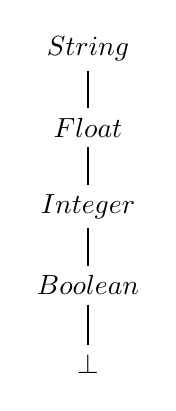
\begin{tikzpicture}

	\node (string)  {$String$};
	\node [below  of=string] (float)  {$Float$};
	\node [below  of=float] (int)  {$Integer$};
	\node [below  of=int] (bool)  {$Boolean$};
	\node [below  of=bool] (bottom)  {$\bot$};
	\draw [thick] (string) -- (float); 
	\draw [thick] (float) -- (int); 
	\draw [thick] (int) -- (bool);
	\draw [thick] (bool) -- (bottom); 
	
	\end{tikzpicture}
\end{center}

In section \ref{concrete} we define $ \mathcal{S} $ to be the set of all possible strings. Here we define the sets $ \mathbb{F}, \mathbb{I}, \mathbb{B} \subseteq \mathcal{S} $ to be the sets of strings that can be interpreted as floating-point numbers, integers and booleans respectively. Then we define a concretization function $ \gamma_{\mathbf{T}}: \mathbf{T} \longrightarrow \mathcal{S} $ for the type lattice as follows: 
\begin{center}
 $ \gamma_{\mathbf{T}}(String) = \mathcal{S} $ \\
 $ \gamma_{\mathbf{T}}(Float) = \mathbb{F} $ \\
  $ \gamma_{\mathbf{T}}(Integer) = \mathbb{I} $ \\
   $ \gamma_{\mathbf{T}}(Boolean) = \mathbb{B} $ \\
    $ \gamma_{\mathbf{T}}(\bot) = \phi $

\end{center}
The operators $ \sqsubseteq_{\mathbf{T}}, \sqcup_{\mathbf{T}}, \sqcap_{\mathbf{T}} $ can be defined using the Hasse diagram above. \\

We define arithmetic operations for the type lattice so that we can evaluate the types of complex expressions. We note that these operations are Python-specific and might need to be redefined for other languages:\\
\hspace*{15mm}$ t_{1} + t_{2}$ = $ \left\{
\begin{array}{ll}
Integer & t_{1} = Boolean \wedge t_{2} = Boolean \\
String & t_{1} = String \wedge t_{2} = String \\
\bot_{\mathbf{T}} & (t_{1} = String \wedge t_{2} \neq String) \vee (t_{1} \neq String \wedge t_{2} = String) \\
t_{1} \sqcup_{\mathbf{T}} t_{2} & otherwise
\end{array} 
\right. $ \\ \\

\hspace*{10mm}$ t_{1} - t_{2}$ = $ \left\{
\begin{array}{ll}
Integer & t_{1} = Boolean \wedge t_{2} = Boolean \\
\bot_{\mathbf{T}} & t_{1} = String \vee  t_{2} = String \\
t_{1} \sqcup_{\mathbf{T}} t_{2} & otherwise
\end{array} 
\right. $ \\ \\

\hspace*{10mm}$ t_{1} \times t_{2}$ = $ \left\{
\begin{array}{ll}
Integer & t_{1} = Boolean \wedge t_{2} = Boolean \\
\bot_{\mathbf{T}} & t_{1} = String \wedge  (t_{2} = String \vee t_{2} = Float) \\
\bot_{\mathbf{T}} & t_{2} = String \wedge  (t_{1} = String \vee t_{1} = Float) \\
t_{1} \sqcup_{\mathbf{T}} t_{2} & otherwise
\end{array} 
\right. $ \\ \\

\hspace*{10mm}$ t_{1} \div t_{2}$ = $ \left\{
\begin{array}{ll}
 \bot_{\mathbf{T}} & t_{1} = Boolean \vee t_{2} = Boolean \\
	Float & otherwise
\end{array} 
\right. $ \\ \\
 
To define the Type Domain, we assume that a static type inference \cite{mostafa} has already been run on the program and that it infers the most generic type for a variable in all execution paths of the program. Our Type Domain aims to track more fine-grained information about the types of variables. We assume that the function $ \mathtt{type}(v) $ returns the type of an expression according to the type inference. Then we proceed to define the Type Domain as follows:  

\begin{center}
	$ \mathrm{TYP} \equiv \mathcal{V} \longrightarrow \mathbf{T}$
\end{center} 

The operators of the Type Domain are all defined point-wise using the underlying type lattice operators. 

\begin{itemize}
	\item An element $ t \in \mathrm{TYP} = \lbrace v \rightarrow typ\ \vert\ v \in \mathcal{V} \wedge typ \in \mathbf{T}  \rbrace $. An element of this domain maps a variable to an element of the type lattice. 
	\item A concretization function $ \gamma_{\mathbf{TYP}} $:
	\begin{itemize} 
		\item We first define a function $ \gamma_{c}: (\mathcal{V} \rightarrow \wp(\mathcal{S})) \longrightarrow \wp(\mathcal{V} \rightarrow \mathcal{S}) $, which transforms a mapping from variable to multiple string values to multiple mappings from a variable to a string value. 
		\item We define an intermediate concretization function $ \gamma'_{\mathbf{TYP}}: \mathrm{TYP} \longrightarrow (\mathcal{V} \rightarrow \wp(\mathcal{S})) $ as follows: $ \gamma'_{\mathrm{TYP}}(f) = \lambda_{x}\cdot \gamma_{\mathbf{T}}(f(x)) $. 
		\item Finally, the concretization function of the Type Domain $ \gamma_{\mathrm{TYP}}: \mathrm{TYP} \longrightarrow \wp(\mathcal{V} \rightarrow \mathcal{S}) $ as the chaining of the two previous functions: $ \gamma_{c} \circ \gamma'_{\mathrm{TYP}}$. It maps every variable to the possible values it can take according to its type. 
	\end{itemize}

\item A partial order $ \sqsubseteq_{\mathrm{TYP}} $: $ t_{1} \sqsubseteq_{\mathrm{TYP}} t_{2} \Longleftrightarrow \forall_{v \in \mathcal{V}} (t_{1}(v) \sqsubseteq_{\mathbf{T}} t_{2}(v))$. For an element of the domain to be smaller than the other, it has to the case that it maps every variable involved in the program to a smaller lattice element than it is mapped in the other element. 


\item A minimum element $ \bot_{\mathrm{TYP}} = \lambda_{x} \cdot \bot_{\mathbf{T}}$. It simply maps every variable to the least element of the type lattice. This represents a type error state. 

\item A maximum element $ \top_{\mathrm{TYP}} = \lambda_{x} \cdot \mathtt{type}(x) $. Since the type inference calculates the most generic type a variable can take, the maximum element of this domain maps every variable to the type computed for it by the type inference. If a variable has a type Float in the type inference, then this it the most generic it can have in all paths of the program and therefore we do not assign it to String but to Float. 

\item A join operator $ \sqcup_{\mathrm{TYP}} $: $ t_{1} \sqcup_{\mathrm{TYP}} t_{2} = \lambda_{x}\cdot t_{1}(x) \sqcup_{\mathbf{T}} t_{2}(x) $. If variable is mapped to two different types in two different paths, then, when these paths are joined, we map the variable to the more \textit{generic} type. That is, the type that is higher in the type lattice Hasse diagram. For example if $ t_{1} = \lbrace x \rightarrow Float \rbrace $ and $ t_{2} = \lbrace x \rightarrow Integer \rbrace $ then $ t_{1} \sqcup _{\mathrm{TYP}} t_{2} = \lbrace x \rightarrow Float \sqcup_{\mathbf{T}} Integer \rbrace = \lbrace x \rightarrow Float \rbrace $

\item A meet operator $ \sqcap_{\mathrm{TYP}} $: $ t_{1} \sqcap_{\mathrm{TYP}} t_{2} = \lambda_{x}\cdot t_{1}(x) \sqcap_{\mathbf{T}} t_{2}(x) $. Using the same example we used for the join,  $t_{1} \sqcap _{\mathrm{TYP}} t_{2} = \lbrace x \rightarrow Float \sqcap_{\mathbf{T}} Integer \rbrace = \lbrace x \rightarrow Integer \rbrace $. We take the type that is lower in the type lattice Hasse diagram. 


\item A backward assignment operator $ \llbracket X:=aexpr \rrbracket(t) = \mathrm{SUBS}_{\mathrm{TYP}}(t, X, aexpr)$ which is described in Algorithm \ref{subsT}. The substitution algorithm evaluates $ aexpr $ and all its sub-expressions and then refines the state $ t $ using this evaluation and the type of $ X $. Looking again at the example, we would like to perform the assignment $ \llbracket y = int(x) \rrbracket(t)$: 
\begin{center}
	\verb|x: str = input()| \\
	\verb|y:int = int(x)|
\end{center}
Considering the example backwards, t is $ \lbrace x \rightarrow String, y \rightarrow Integer \rbrace$ at the very end, with the types inferred by the static type inference. We call the substitution algorithm
 $\mathrm{SUBS}_{\mathrm{TYP}}(t, y, int(x))$ and the following steps ensue:
 \begin{itemize}
 	\item $ value = Integer $, stores the current type of the variable  $ y $. 
 	\item The type of $ y $ is then set to its most generic value according to the type inference, which is $ Integer $. Thus it remains unchanged. 
 	\item The evaluate function is called $ \mathrm{EVAL}_{\mathrm{TYP}}(x, t, \lbrace \rbrace) $ and it returns a map with the evaluation of the expression, $ eval = \lbrace  x \rightarrow String \rbrace $ 
 	\item We use the refinement function to get a more precise constraint on the type of the variable $ x $. The refinement function is called as follows: $ \mathrm{REFINE}_{\mathrm{TYP}}(x, eval,eval[x] \sqcap_{\mathbf{T}} value, t)  = (x, \lbrace  x \rightarrow String \rbrace, String \sqcap_{\mathbf{T}} Integer, t)$. Then maps $ x $ to the meet between its own evaluation and the previously stored $ value $ for $ y $. Therefore $ t $ becomes $ \lbrace  x \rightarrow Integer, y \rightarrow Integer \rbrace$.  
 \end{itemize}
 
\item A filter operator $ \llbracket cond \rrbracket(t) = t $. It does not affect the state.
\item A widening operator $ \nabla_{\mathrm{TYP}} \equiv \sqcup_{\mathrm{TYP}} $. The Type Domain is a finite domain and therefore we do not need a widening operator other than the join. 

\item A special extraction operator, as defined in section \ref{sub-domains} which simply gives the type lattice element corresponding the a variable. $ \mathcal{E}_{\mathrm{TYP}}(t, v)  = t(v) $

We note that since the Type Domain is a non-relational domain, a replacement operator $ \mathcal{R}_{\mathrm{TYP}} $ and a unification operator $ \mathcal{U}_{\mathrm{TYP}} $ do not affect the states. 

\end{itemize}

	
	\begin{algorithm}[t]
		\caption{Substitution algorithm for Type Domain} \label{subsT}
		\begin{algorithmic}
			\Function{$ \mathrm{SUBS}_{\mathrm{TYP}} $} {$t,\  x,\ aexpr $}
			
			\State $ value \gets t(x) $
			\State $ t(x) \gets \mathtt{type}(x) $
			\State $ eval \gets \mathrm{EVAL}_{\mathrm{TYP}}(aexpr,t, empty\ map) $
			\State $ \mathrm{REFINE}_{\mathrm{TYP}}(aexpr, eval, eval[x] \sqcap_{\mathbf{T}} value, t) $
			\State \Return $ t $
			\EndFunction
		\end{algorithmic}
	\end{algorithm}


\begin{algorithm}[t]
	\caption{Expression evaluation for Type Domain} \label{evalT}
	\begin{algorithmic}
		\Function{$ \mathrm{EVAL}_{\mathrm{TYP}} $} {$ expr,t , eval $}
		
		\If {$expr$ is a literal}
		\State $ eval[expr] \gets \verb|type|(literal) $ 
		\State \Return $ eval $
		\EndIf
		
		\If {$ expr \in \mathcal{V}$}
		\State $ eval[expr] \gets \mathtt{type}(expr) \sqcap_{\mathbf{T}} t(expr)$
		\State \Return $ eval $
		\EndIf
		
		\If {$ expr = expr1 \diamond expr2\ \textbf{where}\ \diamond \in \lbrace +, -, \times, \div \rbrace $}
		\State $ eval[expr] \gets \mathrm{EVAL}_{\mathrm{TYP}}(expr1) \diamond \mathrm{EVAL}_{\mathrm{TYP}}(expr2)$
		\State \Return $ eval \sqcap_{\mathbf{T}} \verb|type|(expr) $
		\EndIf
		
		\EndFunction
	\end{algorithmic}
\end{algorithm}

\begin{algorithm}[t]
	\caption{Expression refinement for Type Domain} \label{refineT}
	\begin{algorithmic}
		\Function{$ \mathrm{REFINE}_{\mathrm{TYP}} $} {$ expr, eval, value, t$}
		
		\If {$ expr $ is a literal}
		\State \Return t
		\EndIf
		
		\If {$ expr \in \mathcal{V}$}
		\State $ t(x) \gets eval[expr] \sqcap_{\mathbf{T}} value$
		\State \Return $ t $
		\EndIf
		
		\If {$ expr = expr1 \diamond expr2\ \textbf{where}\ \diamond \in \lbrace +, -, \times, \div \rbrace $}
		\State $ value \gets eval[expr] \sqcap_{\mathbf{T}} value  $
		\State $ refine1 \gets \mathrm{REFINE}_{\mathrm{TYP}}(expr1, eval, value, t) $
		\State $ refine2 \gets \mathrm{REFINE}_{\mathrm{TYP}}(expr2, eval, value, refine1) $
		\State \Return $ refine2 $
		\EndIf
		
		\EndFunction
	\end{algorithmic}
\end{algorithm}

\subsection{The Octagon Domain} \label{octagon}

The Octagon Domain was introduced by Antoine Min\'{e} in \cite{octagon} as a numerical relational domain that can keep track of relations the form $ \pm X \pm Y \geq c $ or of the form $ X \geq c $ where $ X $ and $ Y $ are program variables and $ c $ is a constant. We use the Octagon Domain in our analysis in order to keep track of relations between variables such as $ sequence\_length \leq max\_length $ in Listing 2.1. We refer to \cite{octagon} for the formal definition of the domain and present here the additional functionalities required by our analysis. 

As explained in section \ref{sub-domains}, in order for an existing domain to work with our analysis framework, it needs to define an extraction operator as well as replacement and unification operators in case it is a relational domain. 

For the Octagon Domain, the extraction operator $ \mathcal{E}_{OCT}(v, o)$ simply returns all the constrains in which the variable $ v $ is involved.

\begin{figure} [t]
\begin{lstlisting} [language=Python, caption= Example of Unification] 
	x: int = input()
	if x > 10:
	y: int = int(input())
	if y + x <= 10:
	raise ValueError
	else:
	z: float = float(input())
	if z + x <= 20:
	raise ValueError
\end{lstlisting}
\end{figure}

We define a replacement operator $ \mathcal{R}_{OCT}(o, v, e_{i}) $ for the Octagon Domain, where $ o $ is an octagon, $ v $ is the variable that is being read as input and $ e_{i} $ is an expression in terms of variables $ l_{i} $ that represent the order in which this input-reading statement occurs in the program and constant values. For example if the statement is \verb|v = input() + 3| and it occurs at program point 6, then $ e_{i} $ will be $ l_{6} + 3 $. The operator works by first adding the variables  that occur in $ e_{i} $ to the octagon. These variable have no constraints associated with them at first. Then, assuming the Octagons Domain defines a backward assignment operator, we perform the substitution $ \llbracket v := e_{i} \rrbracket_{OCT} $.

We define the unification operator $ \mathcal{U}_{OCT}(o_{1}, o_{2}) $ where both $ o_{1} $ and $ o_{2} $ are octagons. The operator is applied before every binary operation (join, meet, widening) in the analysis. We assume every element of the Octagon Domain keeps a list of its variables in the order in which they were added during the analysis. When we have two variables that represent inputs read in the same order in two different paths in the analysis, we replace the variable that represents a later program point, with a variable that represents an earlier program point. After this step, if there are variables in $ o_{2} $ which are not in $ o_{1} $, they are added to $ o_{1} $. Note that in this case the operator is asymmetric and needs to be called twice, $ \mathcal{U}_{OCT}(o_{1}, o_{2}) $ and $ \mathcal{U}_{OCT}(o_{2}, o_{1}) $, before every binary operation. 


To illustrate the replacement and unification operators we introduce Listing 2.2. In the then-branch of the if-statement, we read a variable $ y $ and assert the condition $ y + x > 10 $. In the else-branch, we read a variable $ z $ and enforce the condition $ z + x > 20 $. If we trace a backward analysis on this program and employing the $ \mathcal{R}_{OCT} $ we defined earlier in this section, then in the then-branch, we get $\mathcal{R}_{OCT}(\lbrace y + x > 10\rbrace, y, l_{3}) = \lbrace l3 + x > 10 \rbrace$ and similarly in the else-branch we get the relation $ \lbrace l_{7} + x > 20 \rbrace$. A join needs to be performed on these two elements at the head of the if-statement. Since our analysis treats $ l_{3} $ and $ l_{7} $ as different variables, without the unification operator, the join will yield top. 

 As mentioned earlier, our analysis is not concerned with the specific variables representing input values, but rather with the order in which they occur in the list of input values which the program reads in their respective paths. In this example, what matters is that after reading $ x $ we read another variable whose addition to $ x $ had to be greater than 20, otherwise the program will crash. Therefore, for the purpose of our analysis, $ l_{3} $  and $ l_{7} $ should be treated as the same variable when joining the two paths at the head of the if-condition since both of them are read second in their respective paths. We call the unification operator once as follows: $ \mathcal{U}_{OCT}(\lbrace l_{3} + x > 10 \rbrace, \lbrace l_{7} + x > 20 \rbrace) =  \lbrace l_{3} + x > 10 \rbrace$ and then another time switching the operands as follows: $ \mathcal{U}_{OCT}(\lbrace l_{7} + x > 20 \rbrace, \lbrace l_{3} + x > 10 \rbrace) =  \lbrace l_{3} + x > 20 \rbrace$. Then a join can be performed between $ \lbrace l_{3} + x > 10 \rbrace $ and $ \lbrace l_{3} + x > 20 \rbrace $ which will give us $ l_{3} + x > 10 $. 

\subsection{The Character Inclusion Domain} \label{character}
The Character Inclusion Domain, as defined in \cite{character}, is an abstract domain that maps a string into two sets: a set of characters that are certainly included in the string and another set of characters that may be included in the string. 
For a finite alphabet $\mathrm{A}$, we define a character inclusion lattice as follows: 
\begin{itemize}
	\item An element $c \in CI = \lbrace(C, M): C, M \in \wp (\mathrm{A}) \land C \subseteq M \rbrace \cup \bot_{CI}$. This can be understood as an abstraction of a string which certainly contains all the characters in $C$ and is only allowed to contain characters in $ M $.
	
	\item A concretization function $\gamma_{CI}$: $\langle CI, \sqsubseteq_{CI}\rangle  \longrightarrow \langle A^{*}, \subseteq\rangle$ such that \\ $ \gamma_{CI}((C, M)) = \lbrace x\ \vert\ x \in A^{*} \wedge \mathtt{char}(x) \supseteq C \wedge \mathtt{char}(x) \subseteq M \rbrace $, where $ \mathtt{char}(x) $ is a function that returns the set of all characters in a string  $ x $.  An element $ (C, M) $ concertizes to the set of all strings which contain all the characters in $ C $ and which do not contain any characters outside $ M $. 
	
	\item A partial order: $(C_{1}, M_{1}) \sqsubseteq_{CI} (C_{2}, M_{2}) \iff (C_{1} \supseteq C_{2}, M_{1} \subseteq M_{2})$. This order indicates that having a bigger set $ C $ and a smaller set $ M $ means that we represent a smaller set of strings in the concrete domain . For example the element $(\lbrace a \rbrace , \lbrace a,b \rbrace)$ concertizes to $\lbrace a, aa, ab, aaa, aab,... \rbrace$ while the element $(\phi, \lbrace a, b \rbrace)$ concertizes to $\lbrace\varepsilon, a, b, aa, ab, bb,...\rbrace$. The restriction of having $a$ in the certainly included set makes the values $\lbrace \varepsilon, b, bb, bbb,...\rbrace $ disappear from the concretization. 
	
	\item A least element $\bot_{CI}$ which represents a failure state. 
	\item A greatest element $\top_{CI} = (\phi, A) $ which represents a string that can contain any combination of characters from the alphabet. 
	
	\item A join operator: $(C_{1}, M_{1}) \sqcup_{CI} (C_{2}, M_{2}) = (C_{1} \cap C_{2}, M_{1} \cup M_{2})$. The soundness of this operator can be stated as follows: \\ $ \lbrace x\ \vert\ x \in A^{*} \wedge \mathtt{char}(x) \supseteq C_{1} \wedge \mathtt{char}(x) \subseteq M_{1} \rbrace \cup \lbrace x\ \vert\ x \in A^{*} \wedge \mathtt{char}(x) \supseteq C_{2} \wedge \mathtt{char}(x) \subseteq M_{2} \rbrace \subseteq  \lbrace x\ \vert\ x \in A^{*} \wedge \mathtt{char}(x) \supseteq C_{1}\ \cap\ C_{2}\ \wedge\ \mathtt{char}(x) \subseteq M_{1} \cup M_{2} \rbrace \Longleftrightarrow \gamma_{CI}((C_{1}, M_{1})) \cup \gamma_{CI}((C_{2}, M_{2})) \subseteq \gamma_{CI}((C_{1}, M_{1}) \sqcup_{CI} (C_{2}, M_{2}))$. If we have two elements $ (\lbrace a, b \rbrace, \lbrace a, b, c \rbrace) $ and $ (\lbrace a \rbrace, \lbrace a, b, d \rbrace) $ that we would like to join, then we can only say that the resulting element will \textit{certainly} contain the character $ a $ (the intersection of $ C $ sets), but it \textit{may} contain any of the characters $ a,\ b,\ c\ $ or $ d $ (the union of the two $ M $ sets). 
	
	 
	\item A meet operator: $(C_{1}, M_{1}) \sqcap_{CI} (C_{2}, M_{2}) = (C_{1} \cup C_{2}, M_{1} \cap M_{2}) \cup \bot_{CI}$. The bottom is to account for cases when $C_{1} \cup C_{2} \not\subseteq M_{1} \cap M_{2}$. The soundness of this operator can be stated as follows: \\$ \lbrace x\ \vert\ x \in A^{*} \wedge \mathtt{char}(x) \supseteq C_{1} \wedge \mathtt{char}(x) \subseteq M_{1} \rbrace \cap \lbrace x\ \vert\ x \in A^{*} \wedge \mathtt{char}(x) \supseteq C_{2} \wedge \mathtt{char}(x) \subseteq M_{2} \rbrace \subseteq  \lbrace x\ \vert\ x \in A^{*} \wedge \mathtt{char}(x) \supseteq C_{1} \cup C_{2} \wedge \mathtt{char}(x) \subseteq M_{1} \cap M_{2} \rbrace \Longleftrightarrow \gamma_{CI}((C_{1}, M_{1})) \cap \gamma_{CI}((C_{2}, M_{2})) \subseteq \gamma_{CI}((C_{1}, M_{1}) \sqcap_{CI} (C_{2}, M_{2}))$. The meet works in the opposite way to the join. If we have two elements $ (\lbrace a, b \rbrace, \lbrace a, b, c \rbrace) $ and $ (\lbrace a \rbrace, \lbrace a, b, d \rbrace) $ which we would like to meet, we can say that the resulting element will \textit{certainly} contain both $ a $ and $ b $ (the union of the two $ C $ sets) and that it \textit{may} contain only $ a $ and $ b $ (the intersection of the two $ M $ set) as well.  
 	
	\item A concatenation operator: $ ((C_{1}, M_{1}) +_{CI} (C_{2}, M_{2})) = ((C_{1} \cup M_{1}),(C_{2} \cup M_{2}))$. When concatenating two string, the resulting string will \textit{certainly} contain the characters that are certainly included in both strings and \textit{may} contain the characters that may be included in both strings as well. 
	\item A widening operator $\nabla_{CI} \equiv \sqcup_{CI}.$ The widening operator is the same as the join since this domain is a finite domain. 
	
\end{itemize}

	Then we define the Character Inclusion Domain as a mapping from variables to elements of the character inclusion lattice as follows: 
\begin{center}
	$ \mathrm{CHAR} \equiv \mathcal{V} \longrightarrow CI $
\end{center} 
\begin{itemize}
	\item An element $ c \in CHAR = \lbrace v \longrightarrow ci\ \vert\  v \in \mathcal{V} \wedge ci \in CI \rbrace $. Every element in the Character Inclusion Domain maps a variable to an element in the character inclusion lattice. 
	\item A concretization function $ \gamma_{\mathrm{CHAR}} $: 
		\begin{itemize} 
		\item We first define a function $ \gamma_{c}: (\mathcal{V} \rightarrow \wp(\mathcal{S})) \longrightarrow \wp(\mathcal{V} \rightarrow \mathcal{S}) $, which transforms a mapping from variable to multiple string values to multiple mappings from a variable to a string value. 
		\item We define an intermediate concretization function $ \gamma'_{\mathrm{CHAR}}: \mathrm{CHAR} \longrightarrow (\mathcal{V} \rightarrow \wp(\mathcal{S})) $ as follows: $ \gamma'_{\mathrm{CHAR}}(f) = \lambda_{x}\cdot \gamma_{CI}(f(x)) $. 
		\item Finally, we define the concretization function of the Character Inclusion Domain $ \gamma_{\mathrm{CHAR}}: \mathrm{CHAR} \longrightarrow \wp(\mathcal{V} \rightarrow \mathcal{S}) $ as the chaining of the two previous functions: $ \gamma_{c} \circ \gamma'_{\mathrm{CHAR}}$. 
	\end{itemize}

	\item A partial order $ \sqsubseteq_{\mathrm{CHAR}} $: $ c_{1} \sqsubseteq_{\mathrm{CHAR}} c_{2} \Longleftrightarrow \forall_{v \in \mathcal{V}} (c_{1}(v) \sqsubseteq_{CI} c_{2}(v))$.
	\item A minimum element $ \bot_{\mathrm{CHAR}} = \lambda_{x} \cdot \bot_{CI}$. Every variable is mapped to the smallest element in the character inclusion lattice.  
	\item A maximum element $ \top_{\mathrm{CHAR}} = \lambda_{x} \cdot \top_{CI} $. Every variable is mapped to the biggest element of the character inclusion lattice. 
	\item A join operator $ \sqcup_{\mathrm{CHAR}} $: $ c_{1} \sqcup_{\mathrm{CHAR}} c_{2} = \lambda_{x}\cdot c_{1}(x) \sqcup_{CI} c_{2}(x) $ which maps a variable to the joining of the two lattice elements to which it was mapped in $ c_{1} $ and $ c_{2} $.
	 
	\item A meet operator $ \sqcap_{\mathrm{TYP}} $: $ c_{1} \sqcap_{\mathrm{CHAR}} c_{2} = \lambda_{x}\cdot c_{1}(x) \sqcap_{CI} c_{2}(x) $ which maps a variable to the meet of the two lattice elements to which it was mapped in $ c_{1} $ and $ c_{2} $. 
	\item A backward assignment operator $ \llbracket X:=aexpr \rrbracket(c) = \mathrm{SUBS}_{\mathrm{CHAR}}(c, X, aexpr)$ which is described in Algorithm \ref{subsC}. It evaluates $ aexpr $ and all its sub-expressions and refine the state $ c $ with the values computed in this evaluation and the value to which $ X $ was mapped before the assignment is invoked. Meanwhile, $ X $ becomes top.
	
	\item A filter operator $ \llbracket cond \rrbracket(c) =  \mathrm{FILTER}_{\mathrm{CHAR}}(cond, c)$ which is described in Algorithm \ref{filterC}.
	\item A widening operator $ \nabla_{\mathrm{CHAR}} \equiv \sqcup_{\mathrm{CHAR}} $ which is equivalent to the join. 

\end{itemize}
 
As is the case for the Type Domain, the replacement operator $ \mathcal{R}_{\mathrm{CHAR}} $ and a unification operator $ \mathcal{U}_{\mathrm{CHAR}} $ do not produce any changes on the state since this domain is non-relational. 

\begin{algorithm}[H]
	\caption{Substitution algorithm for Character Inclusion Domain} \label{subsC}
	\begin{algorithmic}
		\Function{$ \mathrm{SUBS}_{\mathrm{CHAR}} $} {$c,\  x,\ aexpr $}
		
		\State $ value \gets c(x) $
		\State $ c(x) \gets \top_{CI} $
		\State $ eval \gets emtpy\ map$
		\State $ eval \gets \mathrm{EVAL}_{\mathrm{CHAR}}(aexpr, eval, c) $
		\State $ \mathrm{REFINE}_{\mathrm{CHAR}}(aexpr, eval, eval[x] \sqcap_{CI} value, c) $
		\State \Return $ c $
		\EndFunction
	\end{algorithmic}
\end{algorithm}

\begin{algorithm}[H]
	\caption{Filter algorithm for Character Inclusion Domain} \label{filterC}
	\begin{algorithmic}
		\Function{$ \mathrm{FILTER}_{\mathrm{CHAR}} $} {$cond,\ c$}
		\If {$ cond = (cond1 \wedge cond2) $}
		\State $ c1 \gets \mathrm{FILTER}_{\mathrm{CHAR}}(cond1, c)$
		\State $ c2 \gets \mathrm{FILTER}_{\mathrm{CHAR}}(cond2, c)$
		\State \Return $ c1 \sqcap_{\mathrm{CHAR}} c2$
		\ElsIf {$ cond = (cond1 \vee cond2) $}
		\State $ c1 \gets \mathrm{FILTER}_{\mathrm{CHAR}}(cond1, c)$
		\State $ c2 \gets \mathrm{FILTER}_{\mathrm{CHAR}}(cond2, c)$
		\State \Return $ c1 \sqcup_{\mathrm{CHAR}} c2$
		\ElsIf {$ cond = (expr1 == expr2) $}
		\State $ eval1 \gets empty\ map $
		\State $ eval1 \gets \mathrm{EVAL}_{\mathrm{CHAR}}(expr1, eval1, c) $
		\State $ eval2 \gets empty\ map $
		\State $ eval2 \gets \mathrm{EVAL}_{\mathrm{CHAR}}(expr2, eval2, c) $
		\State $ \mathrm{REFINE}_{\mathrm{CHAR}}(expr1, eval1, eval1[expr1], c)$
		\State $ \mathrm{REFINE}_{\mathrm{CHAR}}(expr2, eval2, eval2[expr2], c)$
				
		\EndIf
		\State \Return $ c $
		\EndFunction
	\end{algorithmic}
\end{algorithm}

\begin{algorithm}[H]
	\caption{Expression evaluation for Character Inclusion Domain} \label{evalC}
	\begin{algorithmic}
		\Function{$ \mathrm{EVAL}_{\mathrm{CHAR}} $} {$ expr, eval, c $}
		
		\If {$expr$ is a literal}
		\State $ eval[expr] \gets (\mathtt{char}(x), \mathtt{char}(x) )$ 
		\State \Return $ eval $
		\EndIf
		
		\If {$ expr \in \mathcal{V}$}
		\State $ eval[expr] \gets c(expr)$
		\State \Return $ eval $
		\EndIf
		
		\If {$ expr = expr1 + expr2$}
		\State $ eval[expr] \gets \mathrm{EVAL}_{\mathrm{CHAR}}(expr1) +_{CI} \mathrm{EVAL}_{\mathrm{CHAR}}(expr2)$
		\State \Return $ eval $
		\EndIf
		
		\EndFunction
	\end{algorithmic}
\end{algorithm}

\begin{algorithm}[H]
	\caption{Expression refinement for Character Inclusion Domain} \label{refineC}
	\begin{algorithmic}
		\Function{$ \mathrm{REFINE}_{\mathrm{CHAR}} $} {$ expr, eval, (C, M), c$}
		
		\If {$ expr $ is a literal}
		\State \Return c
		\EndIf
		
		\If {$ expr \in \mathcal{V}$}
		\State $ c(x) \gets eval[expr] \sqcap_{CI} (C, M)$
		\State \Return $ c $
		\EndIf
		
		\If {$ expr = expr1 + expr2 $}
		\State $ (C, M) \gets eval[expr] \sqcap_{CI} (C, M)  $
		\State $ refine1 \gets \mathrm{REFINE}_{\mathrm{TYP}}(expr1, eval, (\emptyset, M), c) $
		\State $ refine2 \gets \mathrm{REFINE}_{\mathrm{TYPE}}(expr2, eval, (\emptyset, M), refine1) $
		\State \Return $ refine2 $
		\EndIf
		
		\EndFunction
	\end{algorithmic}
\end{algorithm}

\subsection{Tracing the Analysis} \label{trace}
In this section, we trace the static analysis which we have presented in section \ref{analysis} on our running example in Listing \ref{running}. This should give a better understanding of how our analysis works. 

\paragraph{Notation}
We use an element d of the Assumption Domain for this trace where d = ([t, o, c], Q), where t, o and c are elements of the Type Domain, Octagon Domain and Character Inclusion Domain respectively and Q is the stack. For clarity we write each element on a separate line. Also for clarity we assume every variable which is not explicitly written in the constraints of a domain to be set to top in that domain. 

We proceed to trace our analysis backward, starting at the end of the program as follows: \\

\begin{enumerate}
	\item At the beginning of the analysis, the sub-domains have no constraints on the program variables and the stack is initialized with one empty layer :
	\begin{center}
		TYP = $ \top_{TYP} $ \\
		OCT = $ \top_{OCT}$ \\
		CHAR = $ \top_{CHAR} $ \\
		Q = $ 1 \times [\ ] $
	\end{center}
	\item \textbf{Line 29}: we enter the outer loop and also the else 	  branch of the if-statement, so we push two layers on the stack: 
	\begin{center}
		t = $ \top_{TYP} $ \\
		o = $ \top_{OCT}$ \\
		c = $ \top_{CHAR} $ \\
		Q = $ 1 \times [\ ]\ \vert\ 1 \times [\ ]\ \vert\ 1 \times [\ ] $
	\end{center}
	
	However, the raise error statement sets all the sub-domains as well as the stack to bottom: 
	\begin{center}
		t = $ \bot_{TYP} $ \\
		o = $ \bot_{OCT}$ \\
		c = $ \bot_{CHAR} $ \\
		Q = $ \bot_{STACK} $
	\end{center}
	Calling the filter operator with the condition of this branch $ \llbracket $ not(separator == `.' or separator == `\#') $ \rrbracket_{D} $ does not affect the state. 
	
	\item \textbf{Line 27:} we also enter the outer loop and the then branch of the if-statement and therefore push two layers on the stack:
	\begin{center}
		t = $ \top_{TYP} $ \\
		o = $ \top_{OCT}$ \\
		c = $ \top_{CHAR} $ \\
		Q = $ 1 \times [\ ]\ \vert\ 1 \times [\ ]\ \vert\ 1 \times [\ ] $
	\end{center}
	We call the filter operator with the condition of the if-statement $ \llbracket $ separator == `.' or separator == `\#' $ \rrbracket_{D} $ which in turn calls the filter operator of the CHAR element on the two operands of the \textbf{or} operator and then joins the two resulting elements as follows:
	\begin{center}
		$ \llbracket$ separator == `.' $ \rrbracket_{CHAR}(c) = \lbrace separator \rightarrow (\lbrace '.' \rbrace, \lbrace '.' \rbrace) \rbrace $ \\
		$ \sqcup_{CHAR} $ \\
		$ \llbracket$ separator == `\#' $ \rrbracket_{CHAR}(c) = \lbrace separator \rightarrow ( \lbrace '\#' \rbrace, \lbrace '\#' \rbrace) \rbrace $
	\end{center}
	At the end of this step the state is as follows: 
	\begin{center}
		t = $ \top_{TYP} $ \\
		o = $ \top_{OCT}$ \\
		c = 	$ \lbrace separator \rightarrow (\phi, \lbrace '\#', '.' \rbrace) \rbrace $ \\
		Q = $ 1 \times [\ ]\ \vert\ 1 \times [\ ]\ \vert\ 1 \times [\ ] $
	\end{center}
	\item \textbf{Line 26:} We exit the if-statement and pop one layer from the stack. We must then join the states computed in steps 1 and 2 which gives us the following: 
	\begin{center}
		t = $ \top_{TYP} $ \\
		o = $ \top_{OCT}$ \\
		c = 	$ \lbrace separator \rightarrow (\phi, \lbrace '\#', '.' \rbrace) \rbrace $ \\
		Q = $ 1 \times [\ ]\ \vert\ 1 \times [\ ]$
	\end{center}
	\item \textbf{Line 25:} The variable $ separator $ is read as input ans we must store its constraints on the stack. We call the extraction operator to get its corresponding assumption in every domain, then we set separator to top again in all domains: 
	\begin{center}
		$ \mathcal{E}_{TYP} (t, separator) = String $ \\
		$ \mathcal{E}_{OCT} (o, separator) = \top_{O} $ \\
		$ \mathcal{E}_{CHAR}(c, separator) = (\phi, \lbrace '\#', '.' \rbrace) $
	\end{center}
	Then we create an element of the set $ B $ associating the assumptions of the variable wit the current program point:
	\begin{center}
		$ (25, (String, \top_{O}, (\phi, \lbrace '\#', '.' \rbrace))) $
	\end{center}
	We store this element on the top layer of the stack by using the insertion operator $ \mathcal{I}_{I} $:
	\begin{center}
		Q = $ 1 \times [\ ]\ \vert\ \mathcal{I}_{I}(1 \times [\ ], (25, (String, \top_{O}, (\phi, \lbrace '\#', '.' \rbrace))))$ = \\
		$ 1 \times [\ ]\ \vert\ 1 \times [(25, (String, \top_{O}, (\phi, \lbrace '\#', '.' \rbrace)))]$\\
	\end{center}
	
	The final state after this step is: 
	\begin{center}
		t = $ \top_{TYP} $ \\
		o = $ \top_{OCT}$ \\
		c =  $ \top_{CHAR} $\\
		Q = $ 1 \times [\ ]\ \vert\ \mathcal{I}_{I}(1 \times [\ ], (25, (String, \top_{O}, (\phi, \lbrace '\#', '.' \rbrace))))$ = \\
		$ 1 \times [\ ]\ \vert\ 1 \times [(25, (String, \top_{O}, (\phi, \lbrace '\#', '.' \rbrace)))]$\\
	\end{center}
	
	\item \textbf{Line 24:} We enter the inner loop and the else branch of the if-statement starting on line 15, we push 2 layers onto the stack obtained in step 5, but the whole state becomes bottom due to the error statement: 
	\begin{center}
		t = $ \bot_{TYP} $ \\
		o = $ \bot_{OCT}$ \\
		c = $ \bot_{CHAR} $ \\
		Q = $ \bot_{STACK} $
	\end{center}
	\item \textbf{Line 22:} For analyzing the if-statement on lines 15 through 24, we ignore the stack operations resulting from entering the existing multiple nested if-elif-else statement since they do not affect the final result. We, therefore, push one layer onto the stack for entering the inner for-loop:
	\begin{center}
		t = $ \top_{TYP} $ \\
		o = $ \top_{OCT}$ \\
		c =  $ \top_{CHAR} $\\
		Q = $ 1 \times [\ ]\ \vert\ 1 \times [(25, (String, \top_{O}, (\phi, \lbrace '\#', '.' \rbrace)))]\ \vert\ 1 \times [\ ]$\\
	\end{center}
	The statement $ T\_count: int = T\_count + 1 $ calls the assignment operator of $ \llbracket T\_count = T\_count + 1 \rrbracket_{D}(d)$. It does not affect the state. 
	Similar to step 3, we filter using the condition $ base == 'T' $ and we get the following:
	\begin{center}
		t = $ \top_{TYP} $ \\
		o = $ \top_{OCT}$ \\
		c =  $ \lbrace base \rightarrow ('T', 'T') \rbrace $\\
		Q = $ 1 \times [\ ]\ \vert\ 1 \times [(25, (String, \top_{O}, (\phi, \lbrace '\#', '.' \rbrace)))]\ \vert\ 1 \times [\ ]$\\
	\end{center}
	Joining this state with the state obtained from step 6, it remains unchanged. 
	\item \textbf{Line 20:} Similar to the previous step, the assignment $ G\_count = G\_count + 1 $ does not affect the state. Then we apply the filter operator with the condition $ base == 'G' $ to get the following state: 
	\begin{center}
		t = $ \top_{TYP} $ \\
		o = $ \top_{OCT}$ \\
		c =  $ \lbrace base \rightarrow ('G', 'G') \rbrace $\\
		Q = $ 1 \times [\ ]\ \vert\ 1 \times [(25, (String, \top_{O}, (\phi, \lbrace '\#', '.' \rbrace)))]\ \vert\ 1 \times [\ ]$\\
	\end{center}
	Joining this with the state obtained in the previous step we effectively join the last two branches of the if-statement, both of which assume some condition on the variable of $ base $:
	\begin{center}
		c =  $ \lbrace base \rightarrow ('G', 'G') \rbrace $ \\
		$ \sqcup_{CHAR} $ \\
		$ \lbrace base \rightarrow ('T', 'T') \rbrace $ \\
		$ = \lbrace base \rightarrow (\phi,\lbrace 'G', 'T' \rbrace) \rbrace $
	\end{center}
	\item \textbf{Line 18 and 16:} Proceed in a similar manner to the previous two steps, we reach the head of the if-statement on line 15 with the following state: 
	\begin{center}
		t = $ \top_{TYP} $ \\
		o = $ \top_{OCT}$ \\
		c =  $ \lbrace base \rightarrow (\phi, \lbrace'T', 'G', 'C', 'A' \rbrace) \rbrace $\\
		Q = $ 1 \times [\ ]\ \vert\ 1 \times [(25, (String, \top_{O}, (\phi, \lbrace '\#', '.' \rbrace)))]\ \vert\ 1 \times [\ ]$\\
	\end{center}
	\item \textbf{Line 14:} The variable $ base $ is read as input and we must store the assumptions we have collected about it so far. We call the extraction operator to get its corresponding assumption in every domain, then we set $ base $ to top again in all domains: 
	\begin{center}
		$ \mathcal{E}_{TYP} (t, base) = String $ \\
		$ \mathcal{E}_{OCT} (o, base) = \top_{O} $ \\
		$ \mathcal{E}_{CHAR}(c, base) = (\phi, \lbrace'T', 'G', 'C', 'A' \rbrace) \rbrace $
	\end{center}
	Then we create an element of the set $ B $ associating the assumptions of the variable wit the current program point:
	\begin{center}
		$ (14, (String, \top_{O}, (\phi, \lbrace'T', 'G', 'C', 'A' \rbrace) \rbrace)) $
	\end{center}
	We store this element in the top layer of the stack by using the insertion operator $ \mathcal{I}_{I} $:
	\begin{center}
		Q = $ 1 \times [\ ]\ \vert\ 1 \times [(25, (String, \top_{O}, (\phi, \lbrace '\#', '.' \rbrace)))]\ \vert\ \mathcal{I}_{I} (1 \times [\ ], (14, (String, \top_{O}, (\phi, \lbrace'T', 'G', 'C', 'A' \rbrace) \rbrace)))$\\
		= $ 1 \times [\ ]\ \vert\ 1 \times [(25, (String, \top_{O}, (\phi, \lbrace '\#', '.' \rbrace)))]\ \vert\ 1 \times [\ (14, (String, \top_{O}, (\phi, \lbrace'T', 'G', 'C', 'A' \rbrace) \rbrace))]$
	\end{center}
	\item \textbf{Line 13:} We exit the inner loop and thus pop the top layer of the stack. Since this is a pop due to a loop exit, we first replace the multiplier of the top layer with the variable $ sequence\_length $:
	\begin{center}
		$sequence\_length \times [\ (14, (String, \top_{O}, (\phi, \lbrace'T', 'G', 'C', 'A' \rbrace) \rbrace))]$
	\end{center}
	Then we insert it into the layer right below it using $ \mathcal{I}_{I} $, we get the following:
	\begin{center}
		$ t = \top_{TYP} $ \\
		$ o = \top_{OCT} $ \\
		$ c = \top_{CHAR} $ \\
		$ Q = 1 \times [\ ]\ \vert\ 1 \times [\ sequence\_length \times [\ (14, (String, \top_{O}, (\phi, \lbrace'T', 'G', 'C', 'A' \rbrace) \rbrace))], (25, (String, \top_{O}, (\phi, \lbrace '\#', '.' \rbrace)))]$
	\end{center}
	\item \textbf{Lines 9 through 12:} These assignment statements produce no effect on the state since we have no constraints on the variables $ A\_count $, $ C\_count $, $ G\_count $ and $ T\_count $. 
	\item \textbf{Line 7:} The if-statement on lines 7 and 8 adds the constraint $ sequence\_length \leq max\_length $ in the Octagon Domain, the state change as follows:
	\begin{center}
		$ t = \top_{TYP} $ \\
		$ o = \lbrace sequence\_length \leq max\_length \rbrace $\\
		$ c = \top_{CHAR} $ \\
		$ Q = 1 \times [\ ]\ \vert\ 1 \times [\ sequence\_length \times [\ (14, (String, \top_{O}, (\phi, \lbrace'T', 'G', 'C', 'A' \rbrace) \rbrace))], (25, (String, \top_{O}, (\phi, \lbrace '\#', '.' \rbrace)))]$
	\end{center}
	\item \textbf{Line 6:} The variable $ sequence\_length $ is read as input. We call the extraction operator for every domain to get the constraints related to it, while we set the variable to top in all the domains: 
	\begin{center}
		$ \mathcal{E}_{TYP} = Integer $
		$ \mathcal{E}_{OCT} = \lbrace sequence\_length \leq max\_length \rbrace $
		$ \mathcal{E}_{CHAR} = \top $
	\end{center}
	We create an element of the set $ B $ and associate it with the program point 6:
	$ (6, (Integer, \lbrace sequence\_length \leq max\_length \rbrace ), \top) $
	Then we store it on the top layer of the stack using $ \mathcal{I}_{I} $: 
	\begin{center}
		$ Q = 1 \times [\ ]\ \vert\ 1 \times [(6, (Integer, \lbrace sequence\_length \leq max\_length \rbrace ), \top), \ sequence\_length \times [\ (14, (String, \top_{O}, (\phi, \lbrace'T', 'G', 'C', 'A' \rbrace) \rbrace))], (25, (String, \top_{O}, (\phi, \lbrace '\#', '.' \rbrace)))]$
	\end{center}
	
	We then call the replacement operator $ \mathcal{R}_{I} $ on the top layer which introduces the new variable $ l_{6} $ and uses it to replace $ sequence\_length $. The final state after this step is as follows:
	\begin{center}
		$ t = \top_{TYP} $ \\
		$ o = \top_{OCT} $\\
		$ c = \top_{CHAR} $ \\
		$ Q = 1 \times [\ ]\ \vert\ 1 \times [(6, (Integer, \lbrace \mathbf{l_{6}} \leq max\_length \rbrace ), \top), \ \mathbf{l_{6}} \times [\ (14, (String, \top_{O}, (\phi, \lbrace'T', 'G', 'C', 'A' \rbrace) \rbrace))], (25, (String, \top_{O}, (\phi, \lbrace '\#', '.' \rbrace)))]$
	\end{center}
	
	\item \textbf{Line 5:} We exit the outer loop. Similar to step 11, we perform a pop by replacing the multiplier of the top layer with $ number\_of\_sequences $ and inserting it in the layer right below it. We get the following stack: 
	\begin{center}
		$ Q = 1 \times [ number\_of\_sequences \times [(6, (Integer, \lbrace \mathbf{l_{6}} \leq max\_length \rbrace ), \top), \ \mathbf{l_{6}} \times [\ (14, (String, \top_{O}, (\phi, \lbrace'T', 'G', 'C', 'A' \rbrace) \rbrace))], (25, (String, \top_{O}, (\phi, \lbrace '\#', '.' \rbrace)))]] $
	\end{center}
	\item \textbf{Line 3:} Similar to step 13, we add the constraint $ number\_of\_sequences > 0$ to the Octagon Domain, we get the following:
	\begin{center}
		$ t = \top_{TYP} $ \\
		$ o = \lbrace number\_of\_sequences > 0 \rbrace $\\
		$ c = \top_{CHAR} $ \\
		$ Q = 1 \times [ number\_of\_sequences \times [(6, (Integer, \lbrace \mathbf{l_{6}} \leq max\_length \rbrace ), \top), \ \mathbf{l_{6}} \times [\ (14, (String, \top_{O}, (\phi, \lbrace'T', 'G', 'C', 'A' \rbrace) \rbrace))], (25, (String, \top_{O}, (\phi, \lbrace '\#', '.' \rbrace)))]] $
		
	\end{center}
	\item \textbf{Line 2:} Similar to step 14, we extract the constraint on $ max\_length $ and store it on the stack and replace it with $ l_{2} $ in the Octagon Domain. We get the following:
	\begin{center}
		$ t = \top_{TYP} $ \\
		$ o = \lbrace number\_of\_sequences > 0 \rbrace $\\
		$ c = \top_{CHAR} $ \\
		$ Q = 1 \times [ (2, (Integer, \top, \top)), number\_of\_sequences \times [(6, (Integer, \lbrace \mathbf{l_{6}} \leq \mathbf{l_{2}} \rbrace ), \top), \ \mathbf{l_{6}} \times [\ (14, (String, \top_{O}, (\phi, \lbrace'T', 'G', 'C', 'A' \rbrace) \rbrace))], (25, (String, \top_{O}, (\phi, \lbrace '\#', '.' \rbrace)))]] $
	\end{center}
	\item \textbf{Line 1:} Similarly, we extract the constraints on the variable $ number\_of\_sequences$ and store them on the stack, while setting it to top in all the domains, we then replace it with $ l_{1} $ in the stack:
	
	\begin{center}
		$ t = \top_{TYP} $ \\
		$ o = \lbrace number\_of\_sequences > 0 \rbrace $\\
		$ c = \top_{CHAR} $ \\
		$ Q = 1 \times [ (1, (Integer, \lbrace \mathbf{l_{1}} > 0 \rbrace, \top)) ,(2, (Integer, \top, \top)), \mathbf{l_{1}} \times [(6, (Integer, \lbrace \mathbf{l_{6}} \leq \mathbf{l_{2}} \rbrace ), \top), \ \mathbf{l_{6}} \times [\ (14, (String, \top_{O}, (\phi, \lbrace'T', 'G', 'C', 'A' \rbrace) \rbrace))], (25, (String, \top_{O}, (\phi, \lbrace '\#', '.' \rbrace)))]] $
	\end{center}
	
	The final result of our analysis is the following:\\
	$ 1 \times [ $ \\
	$ (1, (Integer, \lbrace \mathbf{l_{1}} > 0 \rbrace, \top)), $ \\
	$(2, (Integer, \top, \top)), $ \\
	$ \mathbf{l_{1}} \times [(6, (Integer, \lbrace \mathbf{l_{6}} \leq \mathbf{l_{2}} \rbrace ), \top), $ \\
	\hspace*{0.5cm} $ \mathbf{l_{6}} \times [\ (14, (String, \top_{O}, (\phi, \lbrace'T', 'G', 'C', 'A' \rbrace) \rbrace))], $ \\
	\hspace*{1cm} $ (25, (String, \top_{O}, (\phi, \lbrace '\#', '.' \rbrace)))]] $
	
\end{enumerate}



\chapter{Implementation} \label{implementation}

We implemented our static analysis and input checker in Python as an extension to the Lyra project \cite{lyra}. We then implemented a plug-in for IntelliJ IDEA that enables the user to use the analysis and checker as a tool. The plug-in implementation is in Java. 



We implement the Assumption Domain described in section \ref{assumption-domain} in a class we call $ AssumptionState $.  The $ AssumptionState $ class has a list of sub-states which represents the sub-domains in the Assumption Domain. The Type Domain already exists as part of Lyra. We implemented separate classes for the Octagon and Character Inclusion domains. For the Octagon domain, we used the Python interface of the ETH Library for Numerical Analysis (ELINA) \cite{singh}. We added extra logic in order to translate the Lyra representation of expressions and conditions into a representation that is compatible with ELINA and also to implement the replacement and unification operators mentioned in section \ref{octagon}. The Character Inclusion domain is implemented as described in section \ref{character} with the addition of support for built-in python functions that perform checks on the characters included in a string such as \verb|isalpha()|, \verb|isalnum()|, \verb|isdecimal()|, \verb|isdigit()|, \verb|islower()| and \verb|isupper()|. 

Every one of the sub-states keeps track of all program variables. If a variable belongs to a type that the domain cannot handle, then its value will always be top in this domain. Therefore, an integer variable will always be mapped to top in the Character Inclusion Domain and a string variable will never have any constraints on it in the Octagon Domain. We require all sub-states to define functions that convert their constraints into JSON object and parse them back from JSON object. We also require every sub-state to implement an input-checking function that, given a input value read from a file, is able to tell whether this value satisfies the constraints that the sub-state represents or not. 

The class $ InputStack $ also has the stack described in section \ref{stack} which implemented as an extension to the already existing $ Stack $ interface in Lyra. We define the pop and push operators for it as well as the structure of individual stack layers. The stack layer is implemented in the class $ InputLattice $ which represents a list of possibly repeated constraints on the input data (see the set $ I $ in section \ref{stack}) and defines a mechanism for recording assumptions on the top layer as well as for joining lists of assumptions from different paths of the analysis. 

Our implementation follows a hierarchy similar to that used in \cite{madelin}. We implement an $ AssumptionController $ class which acts as the entry point for our tool and takes as input the path to a Python code file and an input data file. This class controls three other classes that are in the layer right below it in the hierarchy: $ AssumptionAnalysis $ which extends the Lyra $ Runner  $ class, $ JSONHandler $ and $ InputChecker $. The $ AnalysisAnalysis $ class is responsible for running a backward static analysis on a given Python program. The $ JSONHandler $ class is responsible for writing the assumptions resulting from the analysis into a JSON file and later reading them back from the JSON file. The $ InputChecker $ runs a checking algorithm an a given input file and produces a list of errors present in the file. 


The analysis starts with an instance of the $ AssumptionState $ class set to top and traverses the program paths backward calling the appropriate functions from the class at every step. The final result of the analysis is stored in the stack of the final state and it is of type $ InputLattice $. When the analysis terminates, the controller retrieves the result and passes it to the $ JSONHandler $ class which writes the assumptions into JSON file by calling the functions defined in every sub-state. For subsequent runs of the controller, it checks if the code of the program has been modified and if it has not been modified, it does not run the analysis again but calls the $ JSONHandler $ to read the assumptions for that program from the existing JSON file and convert them back into an $ InputLattice $ object. The assumptions are then passed to the $ InputChecker $ class along with the input file which is required to be checked for errors. The $ InputChecker $ traverses the input file line by line and checks the value in every line against the corresponding assumption by calling the input-checking functions defined in every sub-state. It produces a dictionary which maps a line number in the input file to a $ CheckerError $ object which contains an appropriate error message describing how the value on this line violates an assumption. 

\begin{figure}[H]
	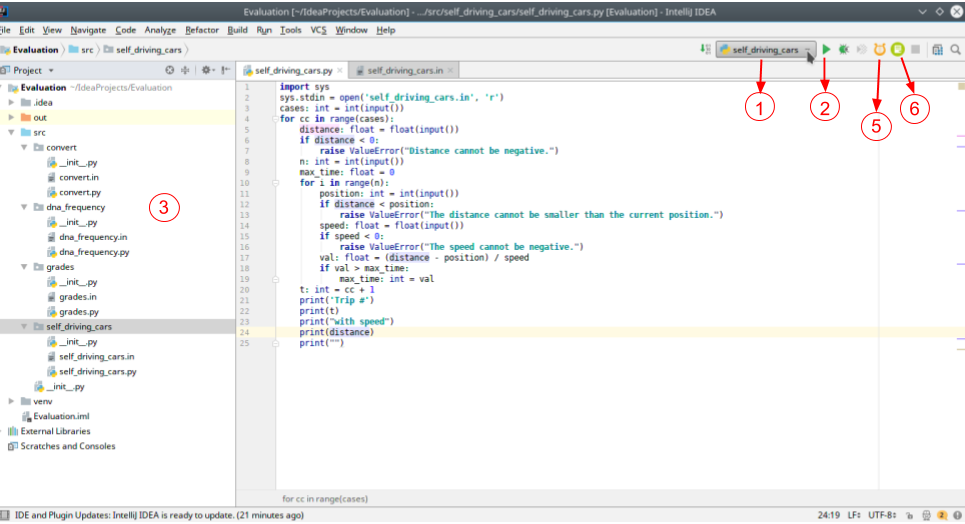
\includegraphics[width=\linewidth]{tool-labeled.png}
	\caption{Screenshot of the IntelliJ IDEA Interface with the Plug-in}
	\label{tool}
\end{figure}

We implement a plug-in for IntelliJ IDEA that allows a user to run our analysis and input checker. The decision to implement such a plug-in was based on feedback received from participants in the user study conducted in \cite{madelin}. The interface which is presented to the user is shown in Figure \ref{tool}. To run the tool on a specific Python program, we must create a run configuration for it and select it from the drop-down menu labeled 1 in the figure. Using the green button labeled 6 we can choose which input data file to check. Then we can run the tool via the button labeled 5 in the figure. The lines which contain errors in the input file will be underlined in red and when the user hovers them with the mouse, an error message will appear. In addition to that, a pop-up message will always appear at the bottom of the screen indicating the location and error message of the first error value in the file. This functionality was added to guide the user step by step in fixing the errors in the file from top to bottom. If the tool cannot detect any more errors in the file, a green pop-up appears at the bottom of the screen indicating so. 
  

\chapter{Evaluation} \label{evaluation}

In this section we present the evaluation of the work done in this thesis. In section \ref{user-study}, we present the methodology and results of a user study we conducted in order to evaluate the usability of our tool. In section \ref{analysis-evaluation}, we present an evaluation of the static analysis we defined in section \ref{analysis}. 

\section{User Study} \label{user-study}
We conducted a user study to evaluate the usability of the tool we developed. We asked ten users, five who have a background in computer science and five who study or work in other fields, to use our tool and give us feedback on how helpful they find it. The methodology of the user study is presented in the next section and the results are presented in section \ref{results}. 

\subsection{Methodology} \label{methodology}

In our user study, we asked our users to do two experiments. For every experiment we presented the user with a programs, accompanied by an input data file which contains some errors that will cause the program to crash, and asked them to try to fix the errors in the data file so that the program runs without crashing. For one experiment they were asked to do this without any help and for the other they were asked to do this with the help of our tool. In the sections below we describe the programs and the input data we use and the procedure of the two experiments.

\subsubsection{Programs and Input Data}

We used four programs in our user study. The programs `Grades' (Listing \ref{grades}) and `Self-Driving Cars' (Listing \ref{cars}) are taken from the user study conducted in \cite{madelin}. The programs `Convert' (Listing \ref{convert}) we obtained from the online sources \cite{convert}. The program `DNA Frequency' (Listing \ref{dna}) we constructed as a possible solution to a slightly modified version of \cite{dna}. The original code of the programs modified so that it can be handled by our analysis. For example, we removed statements that contain lists and function calls. We also added new statements which provide more interesting assumptions on these input data. We constructed the input datasets to contain an average of eight errors per file. The errors we added can be classified into two main types: errors which appear as a result of typing mistakes, such as the number \textbf{6.5}, which represents a grade, being typed as \textbf{6..5} on line 32 in Listing \ref{grades-data}, and errors which result from some garbage values being printed in the data file due to, for example, the conversion of data from one format to another such as the value \textbf{G}, which represents a DNA base, being printed as \textbf{..G} on line 6 in Listing \ref{dna-data}.   \\ 

\subsubsection{Experiments}
As mentioned earlier, we asked every participant in our user study to do two experiments, one after the other. In both experiments the user was presented with a Python program and a text file containing some input data which has errors that will cause the program to crash. They were asked to not change the code of the program but to change the input data, only adding or modifying lines without deleting them, such that the program runs without crashing. The users were presented with an online form that walked them through the experiments step by step. Before starting the experiments, the users were asked to answer some general questions in the form indicating their age, field of study, current occupation and their level of familiarity with programming on five-point Likert scale ranging from 1 to 5, where 1 means "I have never programmed before" and 5 means "I have a strong programming background".  

In both experiments, the form explained to them the task that they are required to perform and then asked them to choose one of the four programs based on their month of birth to ensure some randomness in the experiment. They were handed a sheet of paper containing a brief description of the task the program tries to achieve. In the experiment without the tool, they were given instructions on how to run a Python program in IntelliJ IDEA, while in the experiments with the tool, they were given instructions on how to run the tool and what kind of error messages they should expect to see. Then we allowed the user to work on the problem for eight minutes each. Both the form and the problem descriptions are shown in the Appendix. 

After every task, we asked the users to answer some questions in the form.  For both experiments we asked if they had been able to fix the errors in the input data and how many minutes they spent on this task. For the experiment with the tool, we asked if they were able to run the program without raising any errors. This is to account for the cases were the user was able to fix all the errors detected by the tool, but the tool failed to flag some erroneous data due to imprecision in the analysis.  

These questions were followed by a group of questions on a five-point Likert scale in which the options were: Strongly Disagree, Disagree, Neutral, Agree, Strongly Agree. In both experiments, we asked how frustrated the users felt trying to solve the problems and how understandable they found the error messages printed by the program in the first experiment and displayed by the tool in the second experiment. We added two more questions in the second experiment asking them to rate how user-friendly they found the tool and whether they would rather fix the errors in a data file with or without the help of the tool. 

At the end of the form there were two open-ended questions that aimed to get feedback from the users in their own words. The first questions asked the users what they liked about the tool and the second questions asked them to suggest improvements that they think should be added to the tool. The form as well as the descriptions of the problems can be found in the appendix. 

\subsection{Results} \label{results}

In this section we present some statistics that we gathered from our user study along with some insights that can guide future work on this project. 

The ages of the participants ranges from 19 to 31 with an average of 23.4. Five participants have backgrounds in computer science (one user used the term "informatics" in the form), while two participants have backgrounds in physics, two in environmental engineering and one in mathematics. Six of our participants are bachelor's students, two are master's students, one participant is a postdoctoral researcher and one is a teaching assistant. When asked to rate their familiarity with programming, the majority of participants who rated their experience 4 or above, as expected, have a background in computer science. More details can be seen in Figure \ref{rate}. In all the figures in which we distinguish between computer science and non-computer science participants we label the former as ``CS'' and the later as ``non-CS''. 

\begin{figure}[t]
	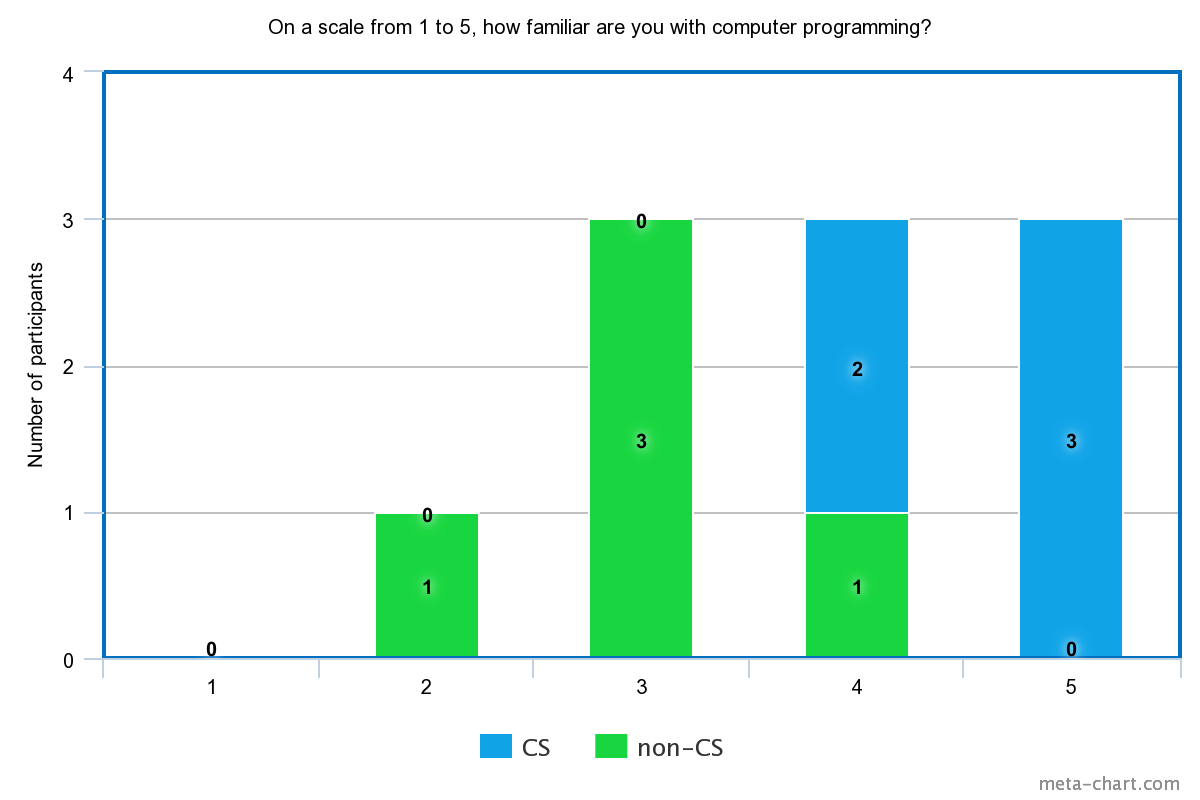
\includegraphics[width=1\linewidth]{rate.png}
	\caption{Answers of: "On a scale from 1 to 5, how familiar are you with computer programming?"}
	\label{rate}
\end{figure}


We found that in the experiment without the tool, only one participant was able to fix all the errors in the input file successfully and it took them 5 and a half minutes. That participant studies computer science and they had rated their familiarity with programming 4 on the five-point scale. All other participants had at least one error in their data files when the assigned 8 minutes of the experiment were over. 

In the second experiment with the tool, 9 out of 10 participants were able to fix all the errors detected by the tool within the 8 minutes of the experiment. The participant who was not able to do so had only one error left in their file at the end of the 8 minutes. They were from a computer science background and had rated their familiarity with programming 5 on the five-point scale. On average, participants without computer science backgrounds took 4.9 minutes, while those with computer science background took 5.7 minutes. We noticed that some participants with computer science background first tried to solve the problem themselves without the help of the tool, while most participants with no background in computer science focused on understanding the error messages of the tool and fixing the input value which they pointed out. The user who could not fix all the errors in the file in the assigned 8 minutes had spent some time trying to solve the problem by examining the code and matching it to the input data. This is a possible explanation for why participants with no background in computer science took less time on average to solve the problem with the tool. 

\begin{figure} [t]
	\centering
	\begin{subfigure}[b]{\textwidth}
		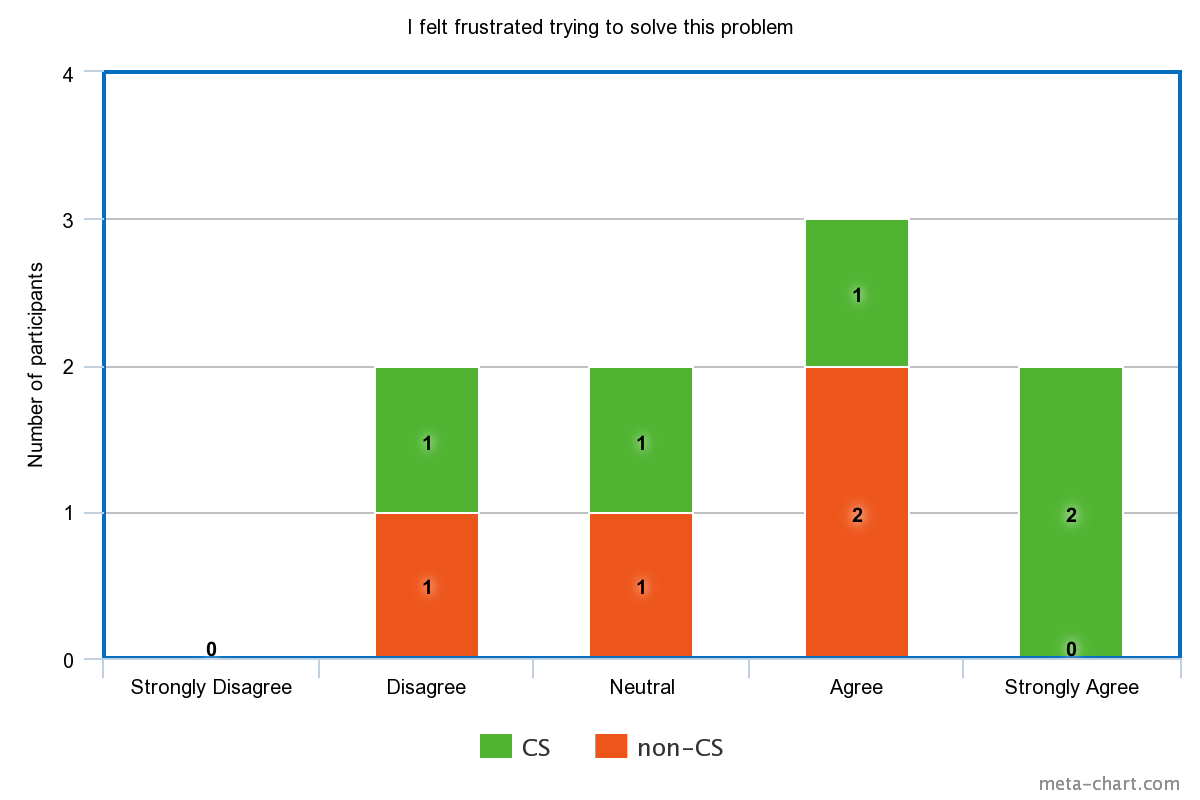
\includegraphics[width=\linewidth]{frust1}
		\caption{Without the tool}
	\end{subfigure} 

	\begin{subfigure}[b]{\textwidth}
		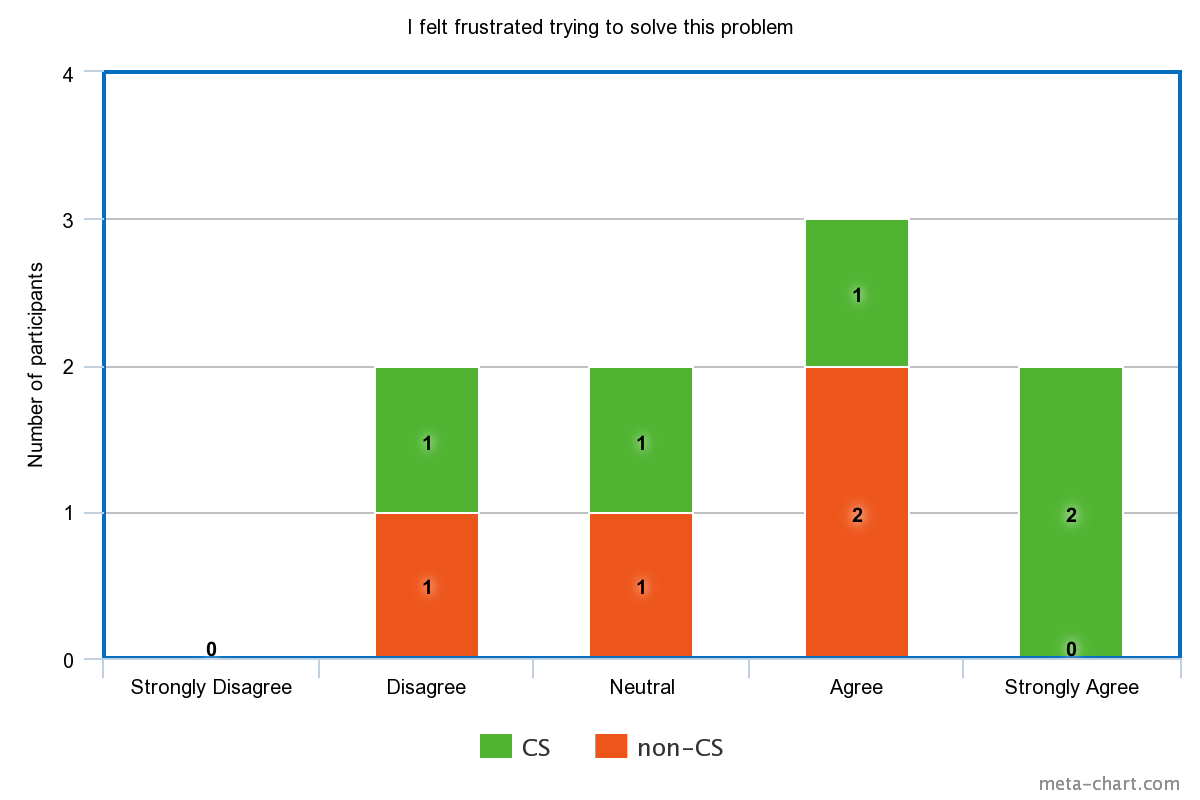
\includegraphics[width=\linewidth]{frust2} 
		\caption{With the tool}
	\end{subfigure}
	\caption{Answers of: "I felt frustrated trying to solve this problem"}
	\label{frustration}%
\end{figure}

The plots in Figure \ref{frustration} show that 6 users reported some level of frustration trying to fix errors in the data without the help of our tool, while only one user reported some level of frustration trying to achieve the same goal with the help of the tool. This, as we expected, shows that our tool created an improvement in the overall debugging experience of the users. An interesting result was that the number of Computer Science participants who felt frustrated trying to debug the data without the help of our tool was less than then the number of non-Computer Science users who felt frustrated performing the same task. A possible explanation for this result is that, as we noticed during the experiments, participants with experience in Computer Science had the expectation that they would be able to examine the code and fix the errors in the data somewhat easily because of their familiarity with programming, unlike non-Computer Science participants who had already expected the task to be challenging.

When asked to state what they liked about the tool, users mentioned that it gave clear and detailed error messages that appeared in the data file and, therefore, they did not have to examine the code to find out the errors in the data. Some of the suggestions that users made to improve the tool were to make it faster, to print the error messages in the console and to highlight which line of code was the source of the error instead of just highlighting the error in the data file. 

From the previous results, we conclude that a tool that guides users through data debugging is a useful tool and helps the users achieve their goals in less time and with less frustration. Some future improvements would be to enhance the performance such that the tool is faster, to introduce an error console in which the users can read the errors all at once without having to scan the data file looking for marked errors and to mark the code lines at which the errors occur instead of just marking the input data lines.  

\begin{lstlisting} [language=Python, label=grades, caption=Code for Program `Grades']
	subject: str = input()
	homeworks: int = int(input())
	students: int = int(input())
	for i in range(students):
		id: str = input()
		sum: float = 0
		max: float = 0
		for j in range(homeworks):
			grade: float = float(input())
			best: float = float(input())
			if grade < 0 or grade > best:
			raise ValueError
			sum: float = sum + grade
			max: float = max + best
		
		average: float = sum / max * 100.0;
		print("Student ID:")
		print(id)
		print("Average homework grade:")
		print(average)
		grade: float = float(input())
		best: float = float(input())
		if grade < 0 or grade > best:
			raise ValueError
		final_grade: float = grade / best * 100.0
		print("Final test grade:")
		print(final_grade)
\end{lstlisting}

\begin{lstlisting} [label=grades-data, caption=Input Data for `Grades']
	CS 101: Introduction to Computer Science
	3
	4
	34-8342
	9
	10
	12
	12
	11
	10
	45
	50
	34-14002
	6
	10
	13
	12
	-9
	10
	51
	50
	31-1234
	5.5
	10
	9
	12
	10#
	10
	-43
	50
	34-2373
	6..5
	10
	11
	12
	7
	10
	48 
\end{lstlisting}

\begin{lstlisting} [language=Python, label=cars, caption=Code for Program `Self-Driving Cars']

cases: int = int(input())
for case in range(cases):
	distance: float = float(input())
	if distance < 0:
		raise ValueError("Distance cannot be negative.")
	n: int = int(input())
	max: float = 0
	for i in range(n):
		position: int = int(input())
		if distance < position:
			raise ValueError("Distance cannot be smaller than the current position.")
		speed: float = float(input())
		if speed < 0:
			raise ValueError("Speed cannot be negative.")
		val: float = (distance - position) / speed
		if val > max:
			max: int = val
	t: int = case + 1
	print("Trip:")
	print(t)
	print("with speed")
	print(distance / max)
	
\end{lstlisting}
\begin{lstlisting} [label=cars-data, caption=Input Data for `Self-Driving Cars]
	4
	10.5
	3
	4
	40
	6
	45.5
	12
	50
	120
	5>>
	25km
	90
	45
	99km/h
	-57
	-123
	76
	130
	1200
	140
	50
	2
	60
	120
	30
	112
	200
	2
	100
	120
	170
\end{lstlisting}

\begin{lstlisting} [language=Python, label=convert, caption= Code Program `Convert'] [H]
items: int = int(input())
if items == 0:
	raise ValueError
for i in range(items):
	name: str = input()
	weight: float = int(input())
	if weight <= 0:
		raise ValueError
	unit: str = input()
	if unit == 'pounds' or unit == 'lb' or unit == 'lbs':
		weight: float = weight * 453.592 * 1e-3
	elif unit == 'ounces' or unit == 'oz' or unit == 'oz.':
		weight: float = weight * 28.35 * 1e-3
	elif unit == 'grams' or unit == 'gms' or unit == 'g':
		weight: float = weight * 1e-3
	elif unit == 'kilograms' or unit == 'kilo' or unit == 'kg':
		pass
	else:
		raise ValueError
	print("Item: " + name)
	print("weight:")
	print(weight)
	print("kg")

	
\end{lstlisting} 

\begin{lstlisting} [label=convert-data, caption=Input Data for `Convert']
	10#
	earphones
	300
	gramx
	stereo set
	0
	kg
	camera tripod
	1@
	qounds
	trolly suitcase
	30
	lbs
	laptop lenovo 5070
	1
	kgs
	laptop lenovo thinkpad
	2>>
	pounds
	12x envelope
	35
	gm.
	bic blue pens 4-piece set
	125
	grams
	travel compass
	50
	grams
	vacuum cleaner
	2#0
	kgs
\end{lstlisting}

\begin{lstlisting}[language=Python, label=dna, caption= Code for Program `DNA Frequency']
	sequences: int = int(input())
	if sequences < 1:
		raise ValueError("Expecting at least one DNA sequence")
	for s in range(sequences):
		length: int = int(input())
		a: int = 0
		c: int = 0
		g: int = 0
		t: int = 0
		for i in range(length):
			base: str = input()
			if base == 'A':
			a: int = a + 1
			elif base == 'C':
			c: int = c + 1
			elif base == 'G':
			g: int = g + 1
			elif base == 'T':
			t: int = t + 1
			else:
			raise ValueError
		separator: str = input()
		if separator == '.' or separator == '#':
			pass
		else:
			raise ValueError
		print("Frequency of A nucleotide:")
		print(a)
		print("Frequency of C nucleotide:")
		print(c)
		print("Frequency of G nucleotide:")
		print(g)
		print("Frequency of T nucleotide:")
		print(t)
		CG_content: float = (c + g) / (a + t + c + g) * 100.0
		print("CG content: ")
		print(CG_content)
		print("%")
\end{lstlisting}

\begin{lstlisting} [label=dna-data, caption=Input Data for `DNA Frequency']
	3..
	10
	A
	O
	C
	..G
	G
	X
	T
	A
	C
	G
	#
	15
	C
	G@
	T
	A
	C
	&C*
	G
	T
	O
	G
	A
	C
	T))
	G
	T
	*
	5
	A
	C
	T
\end{lstlisting}

\section{Evaluation of the Static Analysis} \label{analysis-evaluation}

We evaluated our static analysis using 25 code examples, including slightly modified versions of Listings \ref{grades}, \ref{cars}, \ref{convert}, \ref{dna} which were used in our user study, and an example which we took from \cite{madelin}. The other examples we constructed ourselves in order to test various aspects of our analysis. 

\subsection{Methodology}
Our aim was to measure both the soundness and the precision of our analysis. For every code example, we examined the assumptions inferred by the analysis on each of its inputs and compared it to assumptions that we had computed manually to see whether the analysis was sound and precise. The results are shown in table \ref{table}. The column ``Inputs'' indicates the number of input statements in each program. We consider all the assumptions associated with a single input value to be one assumption. If one domain computes an unsound assumption on an input value, then the whole assumption on this input value is considered unsound and not counted in the ``Sound'' column in our table and, similarly, if one domain computes an imprecise assumption on an input value, then the whole assumption is considered imprecise and counted in the ``Imprecise'' column. 

We added the column ``Source of imprecision'' to gain more insights on how to tune the precision of our analysis and what improvements could be introduced in future work to gain higher precision. The first three sub-columns ``OCT'', ``CHAR'' and ``TYP'' count the number of inputs for which the assumption of the Octagon, Character Inclusion and Type domains were imprecise, respectively. Multiple constraints computed by the Octagon Domain for the same input value are counted as one assumption. The fourth sub-column ``Design'' counts imprecision resulting from limitations in the design of our analysis such as loss of precision due to joins. One imprecise assumption can be counted in more than one of these sub-columns if it has more than one cause. If, for example, both the Type and Octagon domains computed imprecise assumptions on the same input value, then we add one in both the ``OCT'' and ``TYP'' columns.  

\subsection{Results}
Table \ref{table} shows that we counted 73 inputs in all of our examples and that the analysis was sound for all of them, meaning that it did not compute any assumptions that would cause a correct input value to be flagged as an error. There were 29 imprecisions, meaning that for 29 inputs, we could find at least one input value that satisfies the assumptions inferred by our analysis that would still cause the program to crash. 

The Character Inclusion Domain was the least precise domain with 16 imprecise assumptions. We noticed that in 13 of these cases, the loss of precision was due to its inability to distinguish the order or frequency of characters  in a string. For example, in our running example in Listing \ref{running}, it infers the assumption $ (\phi, \lbrace 'A', 'T', 'C', 'G' \rbrace )$ for the variable $ base $. A string such as ``AATC'' would satisfy this assumption, but it would still cause the program to raise an error at runtime. The remaining instances of imprecision were caused by the fact that in our implementation of boolean functions such as \verb|isalpha()|, we infer an assumption such as $ (\phi, \lbrace 'a', 'b', 'c', ...\rbrace ) $ with a ``certainly'' set that is empty, which causes the empty string to satisfy this assumption, while in fact \verb|isalpha("")| evaluates to false. 

The Octagon Domain was imprecise in 7 cases. In 2 cases, the imprecision was due to its inability to detect inequality constraints such as $ n \neq 0 $. There were 3 cases in which the constraints were non-octagonal such as $ a + b < c $. In the remaining 2 cases, information was lost by joining two branches. The Type Domain was imprecise in 4 cases, all of which were because of joining two branches. 

There were 4 imprecisions due to the limitations in the design of our analysis and the fact that if we join two branches and one of them has more input values than the other, we lose some information on the branch with more inputs. We discuss the possibility to overcome this limitation when we discuss future work in section \ref{conclusion}. 

It is evident from our results that, although our analysis has some limitations, a significant improvement in precision can be achieved either by using more domains or by replacing the domains we have used with more powerful ones. For example, if we add the Sign Domain to our analysis, we can capture the 2 assumptions of the form $ n \neq 0 $ which the Octagon Domain misses. The Polyhedra Domain can also capture the 3 constraints of the form $ a + b < c $ which the Octagon Domain cannot capture. If we replace the Character Inclusion Domain with the String Set Domain described in \ref{character}, which keeps track of sets of strings instead of just characters in a string, then for example in Listing \ref{running}, we can say that $ base $ can be only one of exactly four possible values `A', `T', `C' or `G', which achieves a significant increase in precision. 


\begin{table}  \caption{Results of Static Analysis Evaluation} \label{table}
	\let\center\empty
	\let\endcenter\relax
	\centering
	\begin{tabular} {c |c|c|c|c|c|c|c|c}
	Program name & Inputs & Sound & Imprecise & \multicolumn{3}{c}{ Source of imprecision } & & \\
	\hline \\ 
	& & & & OCT & CHAR & TYP & Design \\
	if_condition.py & 2 & 2 & 0 & 0 & 0 & 0 & 0\\
	add.py & 2 & 2 & 0 & 0 & 0 & 0 & 0 \\
	cast.py & 1 & 1 & 0 & 0 & 0 & 0 & 0 \\
	assume1.py & 1 & 1 & 1 & 0 & 1 & 0 & 0\\
	basic.py & 1 & 1 & 1 & 0 & 1 & 0 & 0 \\
	concatenation.py & 2 & 2 & 2 & 0 & 2 & 0 & 0 \\
	merge.py & 3 & 3 & 1 & 0 & 0 & 1 & 1 \\
	must.py & 1 & 1 & 1 & 0 & 1 & 0 & 0 \\
	substitution.py & 3 & 3 & 3 & 0 & 3 & 0 & 0\\
	cars.py & 5 & 5 & 1 & 1 & 0 & 0 & 0 \\
	convert.py & 4 & 4 & 2 & 1 & 1 & 0 & 0 \\
	dna-l.py & 5 & 5 & 2 & 0 & 2 & 0 & 0\\
	food.py & 5 & 5 & 1 & 0 & 0 & 1 & 0 \\
	grades.py & 8 & 8 & 1 & 0 & 1 & 0 & 0 \\
	lost.py & 3 & 3 & 1 & 0 & 0 & 0 & 1  \\
	str_func.py & 2 & 2 & 2 & 0 & 2 & 0 & 0 \\
	triangle_area.py & 3 & 3 & 3 & 3 & 0 & 0 & 0 \\
	type_mix.py & 4 & 4 & 1 & 0 & 1 & 0 & 0 \\
	unification.py & 3 & 3 & 2 & 2 & 0 & 1 & 0 \\
	123.py & 2 & 2 & 0 & 0 & 0 & 0 & 0 \\
	branch.py & 3 & 3 & 1 & 0 & 0 & 1 & 0  \\
	filter.py & 1 & 1 & 0 & 0 & 0 & 0 & 0 \\
	five.py & 3 & 3 & 1 & 0 & 1 & 0 & 0 \\
	loop.py & 3 & 3 & 2 & 0 & 0 & 0 & 2  \\
	merge2.py & 3 & 3 & 0 & 0 & 0 & 0 & 0 \\
	\hline \\
	\textbf{SUM} & 73 & 73 & 29 & 7 & 16 & 4 & 4 & \\
\end{tabular} 

\end{table}

\chapter{Related Work} \label{related}

Many tools and approaches have been developed for the purpose of finding errors in the input data of data science programs. \cite{cleaning} discusses some tools which perform computations on the data itself in order to find and correct errors. For example, data profiling tools collect metadata about a certain attribute and use this metadata to detect errors, while data mining tools are concerned with checking integrity constraints among data attributes. Some tools are domain-specific such as tools that are designed to validate names and addresses and others that specialize in eliminating duplicates. 

CheckCell \cite{checkcell} is an add-in for Microsoft Excel and Google Spreadsheets, which presents an approach called data debugging.  CheckCell works by performing statistical analysis on the input data and pointing out input cells that have a disproportionately large impact on the output, the underlying assumption being that the value of the output changes significantly when an erroneous data value is corrected. As opposed to these works, which require the availability of the input data, our approach analyzes the source code of a program and collects assumptions it makes about its input data and then, whenever the data is available, it can be checked for values that violate these assumptions. 
 
The work done in \cite{madelin} collected assumptions on numerical variables. They designed a type domain and a simple relations domain to keep track of relations between numerical variables such as $ x \leq y $. They used the well-known Interval Domain \cite{cousot} to keep track of ranges which variables are allowed to take. They also used a stack mechanism to store assumptions collected about the input values and designed an input checker to check a data file against the collected assumptions. Their input checker was implemented as a standalone tool. 

The work done in this thesis extends the approach of \cite{madelin} to a generic framework that employs any existing value domain to keep track of assumptions on input values. We also extended the stack mechanism they used for storing assumptions in order to suit the new generic approach for collecting assumptions. We used the Type Domain which was also used in their work to keep track of variable types. For relationships between numerical variables we employed the well-known Octagon Domain, while we used the Character Inclusion Domain to keep track of the characters included in a string. We also implemented an input checker that indicates which values in an input data file violate the assumptions we collected.We implemented a tool as an IDE plug-in which allows users to run our analysis and checker directly on the file they choose. This was done based on recommendations that users gave in a user study conducted in \cite{madelin}.  


\chapter{Conclusion and Future Work} \label{conclusion}
In this thesis, we presented a generic approach to infer assumptions that a program makes about its input data using static analysis. Our approach allows us to make use of any existing value domain to keep track of those assumptions using the Assumption Domain (section \ref{assumption-domain}). We created an instance of this generic domain using three abstract domains: the Type Domain to keep track of assumptions about types, the Octagons Domain to keep track of relational assumptions of the form $ \pm X \pm Y \geq c $ and the Character Inclusion Domain to keep track of assumptions on the characters included in a string. 

We implemented our analysis as an extension to the Lyra project and we designed an input checking algorithm that scans an input data file and flags the values that do not satisfy the assumptions inferred by the analysis. We then integrated our analysis and checker as a tool which we implemented as a plug-in to an IDE. The user can select the program to be analyzed and the input data file to be checked and the plug-in runs the analysis and checker in the background and highlights the errors in the data file directly. 

To evaluate our tool, we conducted a user study in which we took feedback from 10 users on the usability of our tool and the possible improvements that can be added to it. The tool was found useful by the users and helped them find errors in input data in less time and with less frustration. Some possible improvements would be to add an error console to the interface of the tool in order to provide a summary of the errors in the data file, to make the tool faster and to flag the code lines at which the errors happens instead of just flagging the error in the data file. 

We examined the assumptions inferred by our analysis for 25 code examples in order to measure its soundness and precision. Our analysis was sound in all cases. A significant improvement in precision can be achieved by using more powerful domains or employing more domains in our analysis. Another approach to improve precision which was also mentioned in \cite{madelin} would be to extend the analysis to support \textit{conditional assumption}. Instead of performing a regular join between different branches of the analysis and potentially losing some information about one of the branches, we store more than one assumption, each of which holds if a certain condition, for example, a loop or if-statement condition, is met. 
Future work could also include extending the analysis to make it inter-procedural. This would allow for the analysis of more interesting data science program which heavily rely on library function calls in their implementation.  

\appendix
\chapter{Appendix} 

\section{Problem Descriptions of the User Study}

\paragraph{Convert}
A retail store keeps a list of items it sells and their weights. The weights are stored in  the database in the measuring units which the manufacturers placed on the packages: pounds, ounces, grams or kilograms.

The store needs to display the weights of all its items on the website in kilograms. The 
program \textbf{convert.py} helps the store achieve this task, by converting all the weights to kilograms.

\paragraph{DNA Frequency}

There are four possible nitrogenous bases in the DNA: adenine (A), thymine (T), guanine (G) and cytosine (C).

The CG-content of the DNA is the percentage of nucleotides whose nitrogenous base is
either a C or a G. You would like to calculate the CG-content for the a group of DNA
sequences. 

Your IT department sends you the program \textbf{dna_fequency.py} to help you achieve this goal.

\paragraph{Grades}
You are given a  grades.py program that helps you prepare the final grade report for each student in the Introduction to Computer Science course you are teaching.

For each student, it calculates the average homework grade for the entire semester and as well as the final exam grade as a percentage.


\paragraph{Self-driving Cars}

You work as a self-driving cars engineer. You want to test the ability of cars to drive
accident-free in daily traffic, using different routes and considering different numbers of cars on the street.
The program \textbf{self_driving_cars.py} helps you calculate the speed at which a specific car should go, in order to avoid slowing down behind the other cars.

\section{The User Study Form}
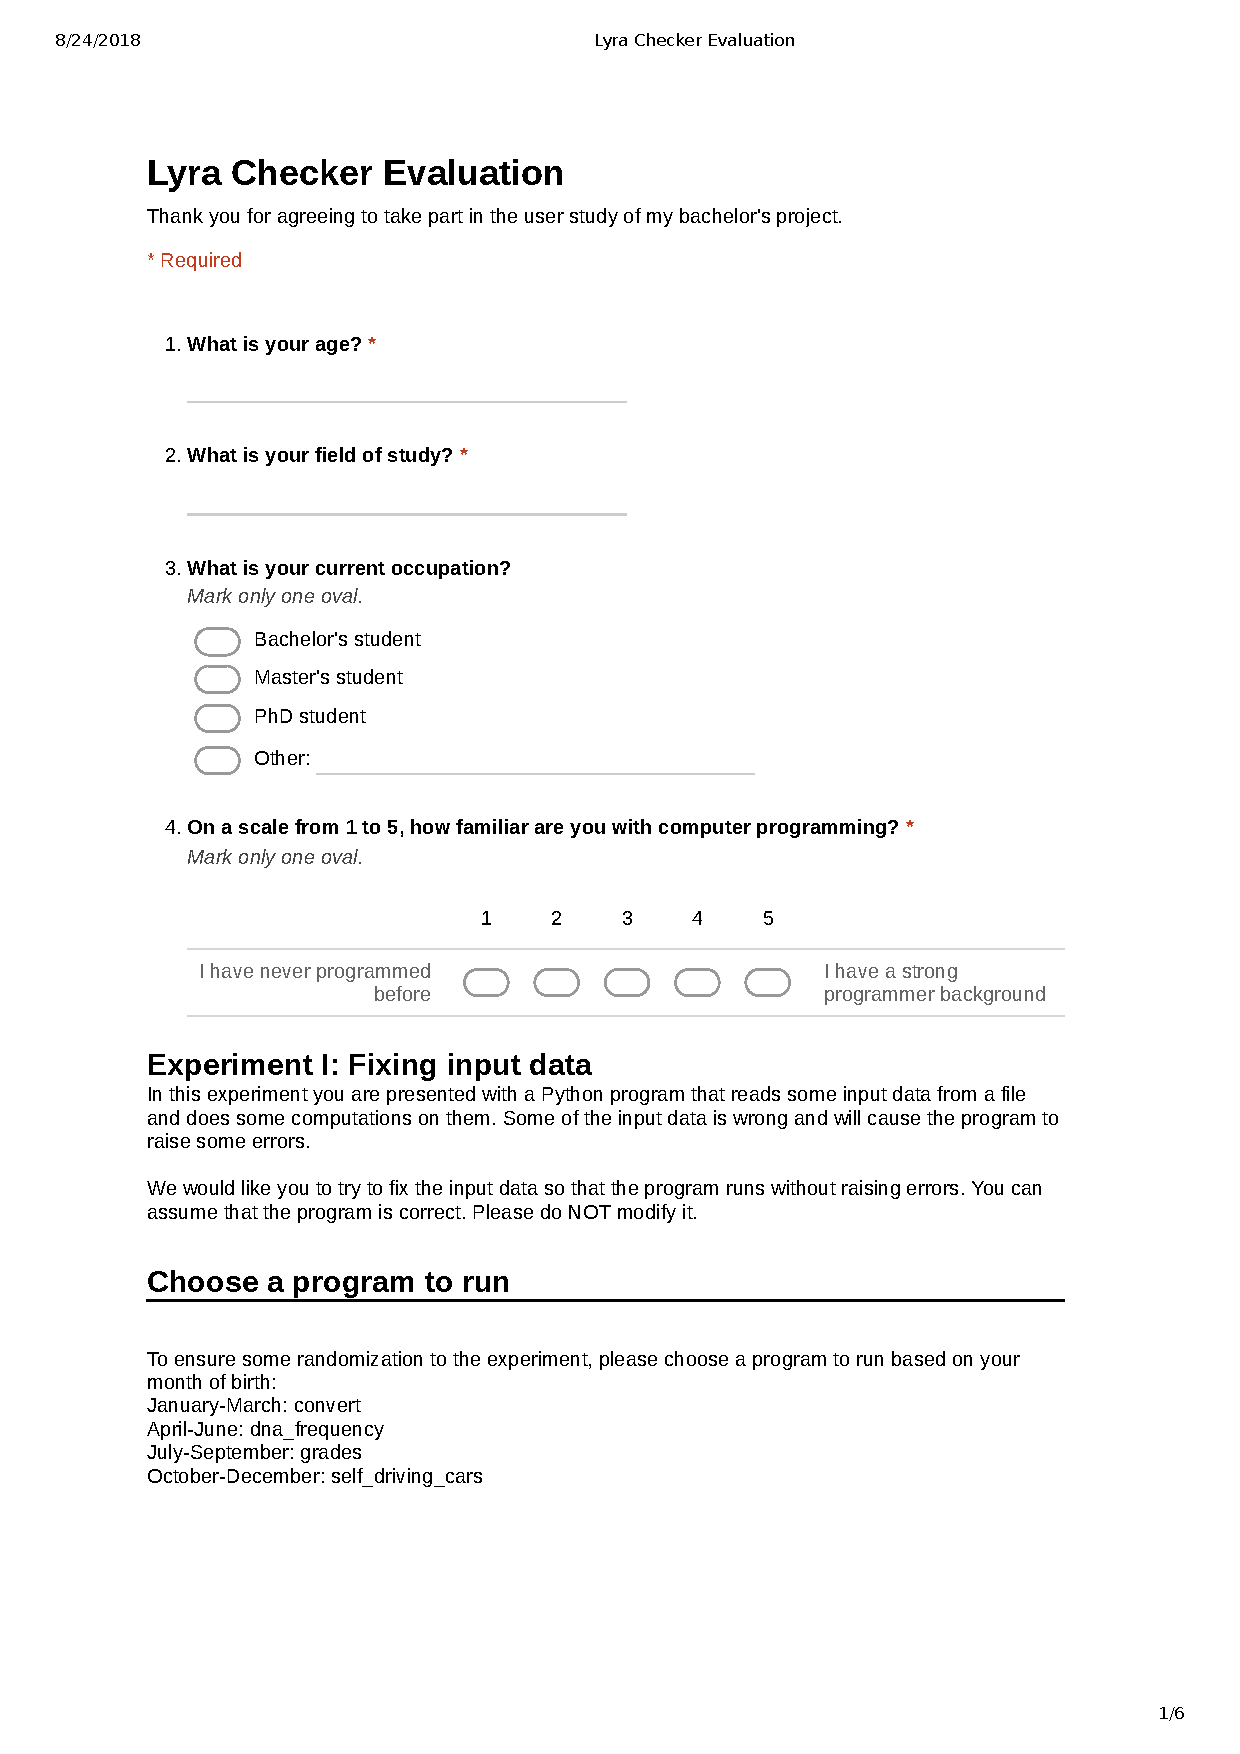
\includepdf[pages={1-6}]{form}

\printbibliography



\end{document}
